
\chapter{Simple applications of the derivative}

 
%64. 
\section{Direction of a curve}
\label{sec:64}

It was shown in \S \ref{sec:32}, %§ 32, p. 31, 
that if

\[
    y = f(x)
\]
is the equation of a curve (see Figure \ref{fig:tangent-example}), 

\begin{figure}[h!]
%\begin{tabular}{cc}
\begin{minipage}{\textwidth}
\begin{center}
%\vspace{1.0 cm}
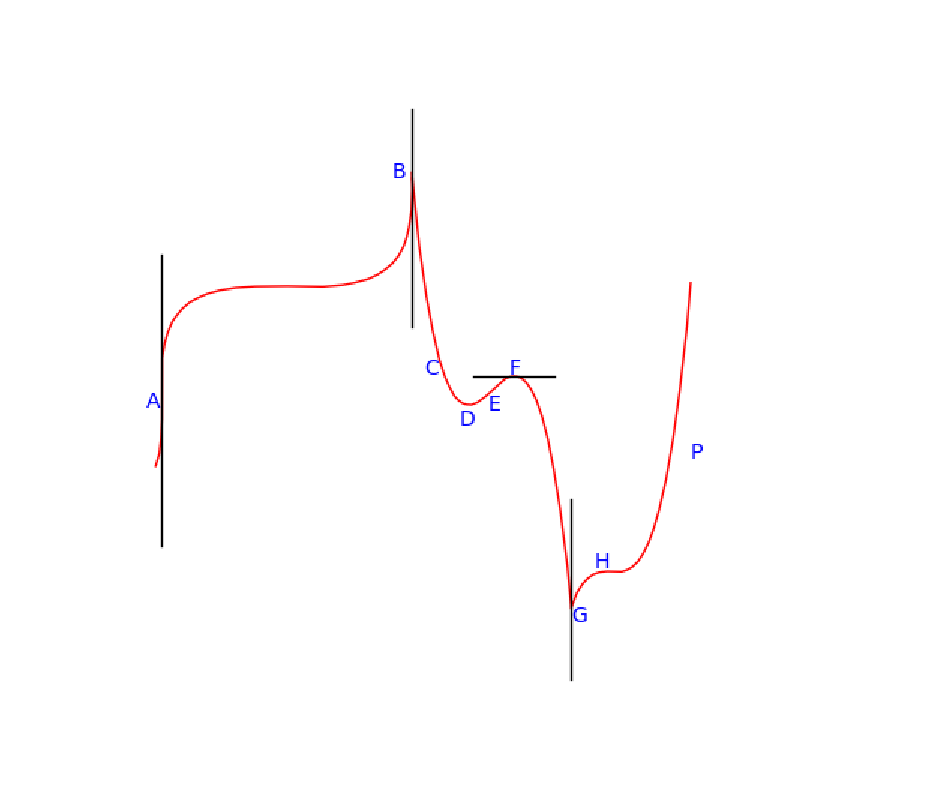
\includegraphics[height=6cm,width=12cm]{curve-tangent.eps}
\end{center}
\end{minipage}
\caption{The derivative = slope of line tangent to the curve.}
\label{fig:tangent-example}
\end{figure}
%sage: f1 = lambda t: [t-sin(t),sin(t)+t]
%sage: p1 = parametric_plot(f1(t), -1, 2*pi, rgbcolor=(1,0,0))
%sage: f2 = lambda t: [t + 2 + 2*RR(pi), 1 + t - t^3 - 7 + 2*RR(pi)]
%sage: p2 = parametric_plot( f2(t), -2, 2, rgbcolor=(1,0,0))
%sage: f3 = lambda t: [t+5+2*RR(pi), t^3-11+2*RR(pi)]
%sage: p3 = parametric_plot( f3(t), -1, 2, rgbcolor=(1,0,0))
%sage: t1 = text('A', (-0.2, 0.0))
%sage: t2 = text('B', (6.0, 6.3))
%sage: t3 = text('C', (6.8, 0.9))
%sage: t4 = text('D', (7.7, -0.5))
%sage: t5 = text('E', (8.4, -0.1))
%sage: t6 = text('F', (8.9, 0.9))
%sage: t7 = text('G', (f3(-1)[0]+0.2, f3(-1)[1]-0.2))
%sage: t8 = text('H', (f3(-1)[0]+0.8, f3(-1)[1]+1.3))
%sage: t9 = text('P', (f3(-1)[0]+3.2, f3(-1)[1]+4.3))
%sage: L1 = line([[0,-4],[0,4]], rgbcolor=(0,0,0))
%sage: L2 = line([[2*pi,2],[2*pi,8]], rgbcolor=(0,0,0))
%sage: L3 = line([[ptD[0]-1,ptD[1]],[ptD[0]+1,ptD[1]]], rgbcolor=(0,0,0))
%sage: L4 = line([[ptG[0],ptG[1]-2],[ptG[0],ptG[1]+3]], rgbcolor=(0,0,0))
%sage: show(p1+p2+p3+t1+t2+t3+t4+t5+t6+t7+t8+t9+L1+L2+L3+L4,axes=False)

\noindent
then

\[
\frac{dy}{dx}\ =\ \tan\ \tau\ =\ {\rm slope\ of\ line\ 
tangent\ to\ the\ curve\ at\ any\ point\ } P.
\]
The direction of a curve at any point is defined to 
be the same as the direction of the line tangent to the 
curve at that point. From this it follows at once that

\[
    \frac{dy}{dx}\ =\ \tan\ \tau\ = \ {\rm slope\ of\ the\ 
curve\ at\ any\ point\ } P. 
\]
At a particular point whose coordinates are known we write

\[
  \left [ \frac{dy}{dx} \right ]_{x=x_1, y=y_1}\ = 
\ {\rm slope\ of\ the\ curve\ (or\ tangent)\ at\ point\ } (x_1,y_1).
\]
At points such as D, F, H, where the curve (or tangent) 
is parallel to the axis of $x$, $\tau = 0^o$,
therefore $\frac{dy}{dx} = 0$.

At points such as A, B, G, where the curve (or tangent) is 
perpendicular to the axis of $x$, $\tau = 90^o$,
therefore $\frac{dy}{dx} = \infty$.

At points such as E, where the curve is rising\footnote{When 
moving from left to right on curve.},

\[
\tau \ = \ {\rm an\ acute\ angle;\ therefore\ }
\frac{dy}{dx}\ =\ {\rm a\ positive\ number}.
\]
The curve (or tangent) has a positive slope to the left of B, 
between D and F, and to the right of G in 
Figure \ref{fig:tangent-example}. %% new
At points such as C, where the curve is falling,

\[
\tau \ = \ {\rm an\ obtuse\ angle;\ therefore\ }
\frac{dy}{dx}\ =\ {\rm a\ negative\ number}.
\]
The curve (or tangent) has a negative slope between B and D, 
and between F and G.


\begin{example}
\label{ex:64}
{\rm
Given the curve $y = \frac{x^3}{3} - x^2 + 2$ (see 
Figure \ref{fig:tangent-example2}).

(a) Find $\tau$ when $x = 1$.

(b) Find $\tau$ when $x = 3$.

(c) Find the points where the curve is parallel to % OX.
the $x$-axis. % new

(d) Find the points where $\tau = 45^o$.

(e) Find the points where the curve is parallel to the 
line $2x - 3y = 6$. %(line AB).

\begin{figure}[h!]
%\begin{tabular}{cc}
\begin{minipage}{\textwidth}
\begin{center}
%\vspace{1.0 cm}
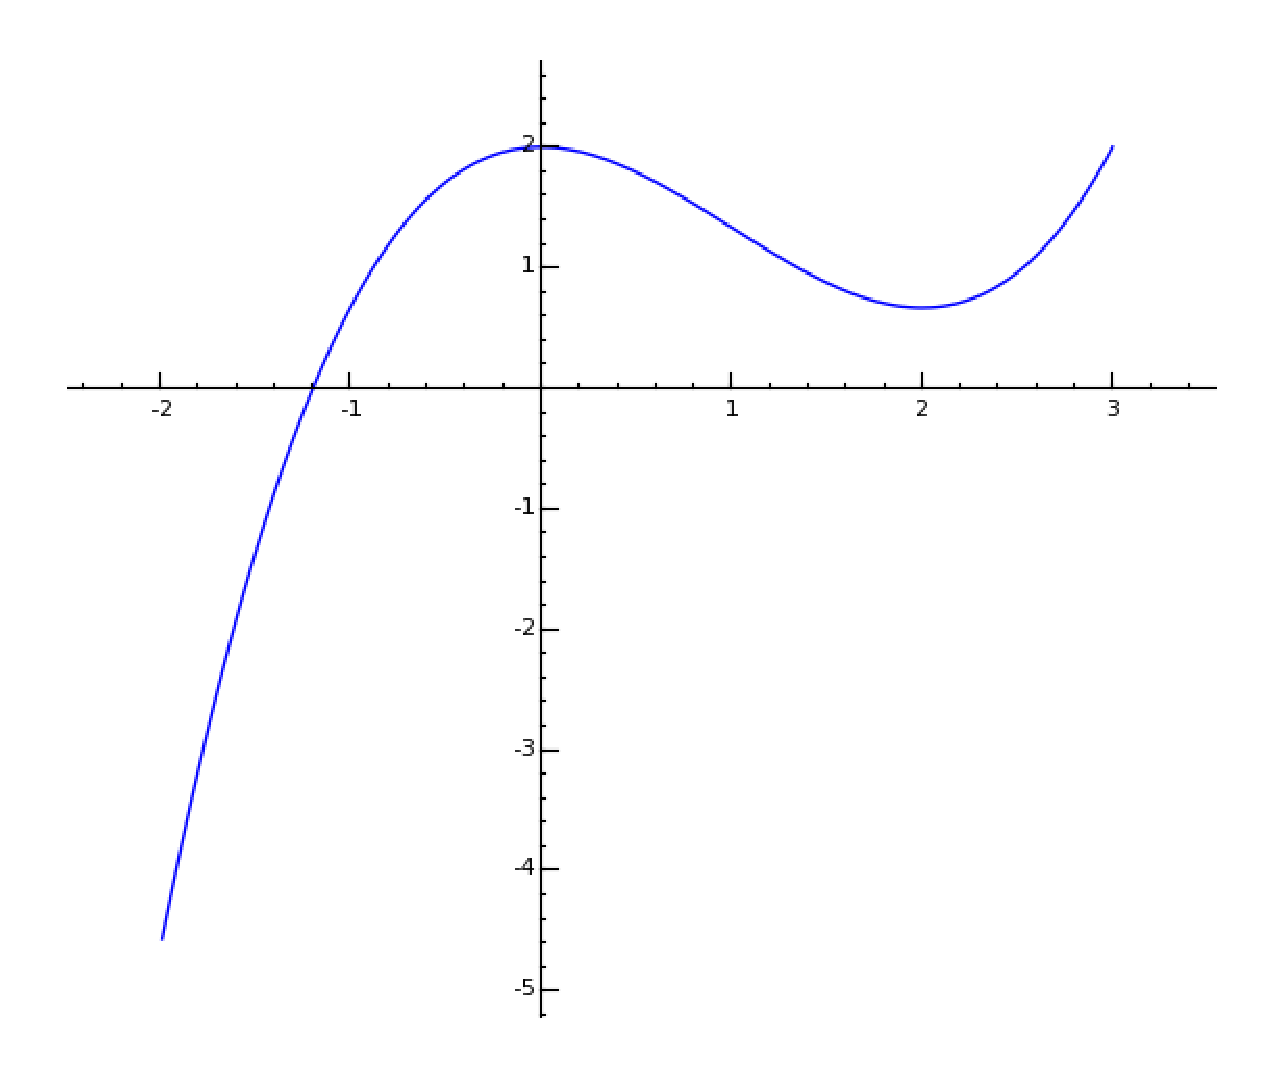
\includegraphics[height=5cm,width=7cm]{tangent-examples2.eps}
\end{center}
\end{minipage}
\caption{The graph of $y = \frac{x^3}{3} - x^2 + 2$.}
\label{fig:tangent-example2}
\end{figure}
%sage: x = var("x")
%sage: f = x^3/3 - x^2 +2
%sage: f.diff()
%x^2 - 2*x
%sage: P = plot(f,-2,3)
%sage: show(P)

Differentiating, $\frac{dy}{dx} = x^2 - 2x$ = slope at any point.

(a) $\tan \tau = \left [ \frac{dy}{dx} \right ]_{x=1} = 1 - 2 = -1$; 
therefore $\tau = 135^o
=3\pi/4$. % new

(b) $\tan \tau = \left [ \frac{dy}{dx} \right ]_{x=3} = 9 - 6 = 3$; 
therefore $\tau = \arctan\, 3 = 1.249...$. 

(c) $\tau = 0^o$, $\tan \tau = \frac{dy}{dx} = 0$; 
therefore $x^2 - 2x = 0$. Solving this equation, 
we find that $x = 0$ or $2$, giving points C and D where the 
curve (or tangent) is parallel to % OX 
the $x$-axis.

(d) $\tau = 45^o$, $\tan \tau = \frac{dy}{dx} = 1$; 
therefore $x^2 - 2x = 1$. Solving, we get 
$x = 1 \pm \sqrt{2}$, giving two points where the slope of 
the curve (or tangent) is unity.

(e) Slope of line = $\frac{2}{3}$; therefore $x^2 - 2x = \frac{2}{3}$. 
Solving, we get $x = 1 \pm \sqrt{\frac{5}{3}}$, giving points E 
and F where curve (or tangent) is parallel to %line AB.
$2x - 3y = 6$.
}
\end{example}

Since a curve at any point has the same direction as 
its tangent at that point, the angle between two curves 
at a common point will be the angle between their tangents at 
that point.

\begin{example}
{\rm
Find the angle of intersection of the circles

(A) $x^2 + y^2 - 4x = 1$,

(B) $x^2 + y^2 - 2y = 9$.

Solution. Solving simultaneously, we find the 
points of intersection to be $(3, 2)$ and $(1, -2)$.
%sage: x = var("x")
%sage: y = var("y")
%sage: F = x^2 + y^2 - 4*x - 1
%sage: G = x^2 + y^2 - 2*y - 9
%sage: solve([F == 0,G == 0],x,y)
%[[x == 1, y == -2], [x == 3, y == 2]]
This can be verified ``by hand'' or using the \sage\ {\tt solve}
command:


\vskip .1in

\begin{Verbatim}[fontsize=\small,fontfamily=courier,fontshape=tt,frame=single,label=\sage]

sage: x = var("x")
sage: y = var("y")
sage: F = x^2 + y^2 - 4*x - 1
sage: G = x^2 + y^2 - 2*y - 9
sage: solve([F == 0,G == 0],x,y)
[[x == 1, y == -2], [x == 3, y == 2]]

\end{Verbatim}
\vskip .1in

\noindent

\begin{figure}[h!]
%\begin{tabular}{cc}
\begin{minipage}{\textwidth}
\begin{center}
%\vspace{1.0 cm}
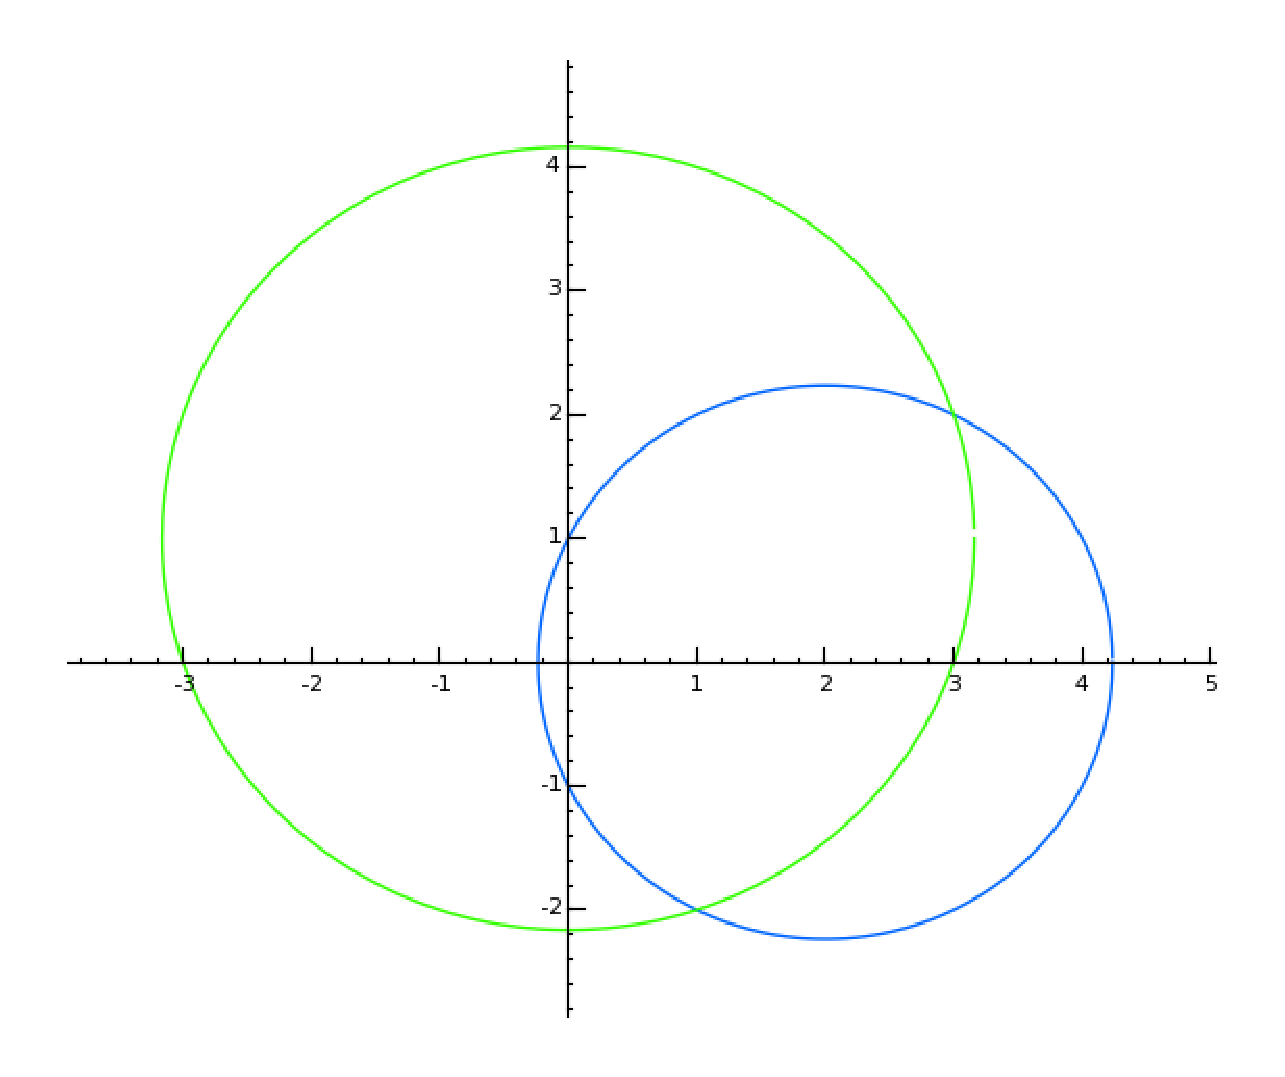
\includegraphics[height=5cm,width=6cm]{circles.eps}
\end{center}
\end{minipage}
\caption{The graphs of $x^2 + y^2 - 4x = 1$, $x^2 + y^2 - 2y = 9$.}
\label{fig:circles}
\end{figure}
%sage: t = var("t")
%sage: P1 = parametric_plot( (sqrt(5)*cos(t)+2, sqrt(5)*sin(t)), 0, 2*pi, rgbcolor=hue(0.6) )
%sage: P2 = parametric_plot( (sqrt(10)*cos(t), sqrt(10)*sin(t)+1), 0, 2*pi, rgbcolor=hue(0.3) )
%sage: show(P1+P2)

Using (A), formulas in \S \ref{sec:63} give
$\frac{dy}{dx} 	= \frac{2 - x}{y}$. Using (B), formulas in 
\S \ref{sec:63} give $\frac{dy}{dx} 	= \frac{x}{1 - y}$.
Therefore,
\[
\left [ \frac{2 - x}{y} \right ]_{x = 3, y = 2} 	
= -\frac{1}{2} =\ {\rm slope\ of\ tangent\ to\ (A)\ at\ } (3, 2).
\]
\[
\left [ \frac{x}{1 - y} \right ]_{x = 3, y = 2} 	= - 3 
=\ {\rm slope\ of\ tangent\ to\ (B)\ at\ }(3, 2).
\]
We can check this %(continuing our \sage session above),
%using the commands\footnote{These commands assume that if 
%$y$ is defined as a function of $x$ by an algebraic expression
%$f(x,y)=0$ then $y'=-f_x(x,y)/f_y(x,y)$, where $f_x$ is the
%partial derivative of $f$ with respect to $x$ and $f_y$ is the
%partial derivative $f$ with respect to $y$. For this example, 
%these formulas will be simply assumed and not proven in Calculus III.}:
%
%\begin{Verbatim}[fontsize=\small,fontfamily=courier,fontshape=tt,frame=single,label=\sage]
%
%sage: FDy = -diff(F,x)/diff(F,y); FDy; FDy(3,2)
%(4 - 2*x)/(2*y)
%-1/2
%sage: GDy = -diff(G,x)/diff(G,y); GDy; GDy(3,2)
%-2*x/(2*y - 2)
%-3
%
%\end{Verbatim}
%\vskip .1in
%
%\noindent
%Here we used $FDy$ to denote the derivative of $y$ with respect to 
%$x$ in the equation $F(x,y)=0$, so $FDy(3,2)$ denotes
%$\frac{dy}{dx}|_{x = 3, y = 2}$ for that curve.
%Likewise, $GDy$ denotes the derivative 
%of $y$ with respect to $x$ in the equation $G(x,y)=0$.
using the commands

\begin{Verbatim}[fontsize=\small,fontfamily=courier,fontshape=tt,frame=single,label=\sage]

sage: x = var("x")
sage: y = function("y",x)
sage: F = x^2 + y^2 - 4*x - 1
sage: F.diff(x)
2*y(x)*diff(y(x), x, 1) + 2*x - 4
sage: solve(F.diff(x) == 0, diff(y(x), x, 1))
[diff(y(x), x, 1) == (2 - x)/y(x)]
sage: G = x^2 + y^2 - 2*y - 9
sage: G.diff(x)
2*y(x)*diff(y(x), x, 1) - 2*diff(y(x), x, 1) + 2*x
sage: solve(G.diff(x) == 0, diff(y(x), x, 1))
[diff(y(x), x, 1) == -x/(y(x) - 1)]

\end{Verbatim}
\vskip .1in

\noindent

The formula for finding the angle between two lines whose 
slopes are $m_1$ and $m_2$ is

\[
\tan\theta = \frac{m_1 - m_2}{1 + m_1 m_2},
\]
by item 55, \S \ref{sec:1}.
Substituting, 
$\tan \theta = \frac{-\frac{1}{2} + 3}{1 + \frac{3}{2}} = 1$; 
therefore $\theta = \pi/4= 45^o$. 
This is also the angle of intersection at the point $(1, -2)$.

}
\end{example}

\section{Exercises}

The corresponding figure should be drawn in each of the following 
examples:

\begin{enumerate}

\item
%1
Find the slope of 
$y = \frac{x}{1 + x^2}$ at the origin. 

Ans. $1 = \tan\, \tau$.

\item
%2
What angle does the tangent to the curve 
$x^2y^2 = a^3(x + y)$ at the origin make with the %axis of X? 
$x$-axis?

Ans. $\tau = 135^o=3\pi/4$.

\item
%3
What is the direction in which the point generating the 
graph of $y = 3x^2 - x$ tends to move at the instant when $x = 1$? 

Ans. Parallel to a line whose slope is $5$.

\item
%4
Show that $\frac{dy}{dx}$ (or slope) is constant for a straight line.

\item
%5
Find the points where the curve $y = x^3 - 3x^2 - 9x + 5$ 
is parallel to the %axis of X. 
$x$-axis.

Ans. $x = 3$, $x = -1$.

\item
%6
At what point on $y^2 = 2x^3$ is the slope equal to $3$? 

Ans. $(2, 4)$.

\item
%7
At what points on the circle $x^2 + y^2 = r^2$ is the 
slope of the tangent line equal to $-\frac{3}{4}$? 

Ans. $\left ( \pm \frac{3r}{5}, \pm \frac{4r}{5} \right )$

\item
%8
Where will a point moving on the parabola $y = x^2 - 7x + 3$ 
be moving parallel to the line $y = 5x + 2$? 

Ans. $(6, -3)$.

\item
%9
Find the points where a particle moving on the circle 
$x^2 + y^2 = 169$ moves perpendicular to the line 
$5x + 12y = 60$. 

Ans. $(\pm 12, \mp 5)$.

\item
%10
Show that all the curves of the system 
$y = \log\, kx$ have the same slope; i.e. the slope is independent of $k$.

\item
%11
The path of the projectile from a mortar cannon 
lies on the parabola $y = 2x - x^2$; the unit is 1 mile, %OX 
the $x$-axis % new
being horizontal and %OY 
the $y$-axis % new
vertical, and the origin being the point of projection. 
Find the direction of motion of the projectile

(a) at instant of projection;

(b) when it strikes a vertical cliff $\frac{3}{2}$ miles distant.

(c) Where will the path make an inclination of $45^o=\pi/4$ 
with the horizontal?

(d) Where will the projectile travel horizontally?

Ans. (a) $\arctan\, 2$; (b) $135^o=3\pi/4$; 
(c) $(\frac{1}{2}, \frac{3}{4})$; (d) $(1, 1)$.

\item
%12
If the cannon in the preceding example was situated on a 
hillside of inclination $45^o=\pi/4$, at what angle would 
a shot fired up strike the hillside? 

Ans. $45^o=\pi/4$.

\item
%13
At what angles does a road following the line 
$3y - 2x - 8 = 0$ intersect a railway track following the 
parabola $y^2 = 8x$? 

Ans. $\arctan \frac{1}{5}$, and $\arctan \frac{1}{8}$.

\item
%14
Find the angle of intersection between the parabola $y^2 = 6x$ 
and the circle $x^2 + y^2 = 16$. 

Ans. $\arctan \frac{5}{3} \sqrt{3}$.

\item
%15
Show that the hyperbola $x^2 - y^2 = 5$ and the ellipse 
$\frac{x^2}{18} + \frac{y^2}{8} = 1$ intersect at right angles.

\item
%16
Show that the circle $x^2 + y^2 = 8ax$ and the cissoid 
$y^2 = \frac{x^3}{2a - x}$
\index{curve! cissoid}

(a) are perpendicular at the origin;

(b) intersect at an angle of $45^o=\pi/4$ at two other points.

\item
%17
Find the angle of intersection of the parabola 
$x^2 = 4ay$ and the Witch of Agnesi,
 $y = \frac{8a^3}{x^2 + 4a^2}$. 
\index{curve! Witch of Agnesi}

Ans. $\arctan\, 3 = 71^o33' = 1.249...$.

For the interesting history of this curve, see for example
\newline
\url{http://en.wikipedia.org/wiki/Witch\_of\_Agnesi}.

\item
%18
Show that the tangents to the Folium of Descartes,
$x^3 + y^3 = 3axy$ at the points where it meets the parabola 
$y^2 = ax$ are parallel to the %axis of Y.
$y$-axis.

For some
history of this curve, see for example
\newline
\url{http://en.wikipedia.org/wiki/Folium\_of\_Descartes}.

\item
%19
At how many points will a particle moving on the curve 
$y = x^3 - 2x^2 + x - 4$ be moving parallel to the %axis of X? 
$x$-axis? What are the points? 

Ans. Two; at $(1,-4)$ and $(\frac{1}{3}, -\frac{104}{27})$.

\item
%20
Find the angle at which the parabolas $y = 3x^2-1$ and 
$y = 2x^2 + 3$ intersect. 

Ans. $\arctan \frac{4}{97}$.

\item
%21
Find the relation between the coefficients of the 
conics $a_1x^2 + b_1y^2 = 1$ and $a_2x^2 + b_2y^2 = 1$ when they 
intersect at right angles. 

Ans. $\frac{1}{a_1} - \frac{1}{b_1} = \frac{1}{b_2} - \frac{1}{b_2}$.

\end{enumerate}

%65. 
\section{Equations of tangent and normal lines}
\label{sec:65}
% section name was too long for latex headers

Full section title: % new
{\it Equations of tangent and normal lines, lengths of subtangent 
and subnormal. Rectangular coordinates.}

The equation of a straight line passing through the 
point $(x_1,y_1)$ and having the slope $m$ is

\[
   y-y_1 = m(x-x_1)
\]
(this is item 54, \S \ref{sec:1}). % 54, (c), p. 3 [§ 1] 

\begin{figure}[h!]
%\begin{tabular}{cc}
\begin{minipage}{\textwidth}
\begin{center}
%\vspace{1.0 cm}
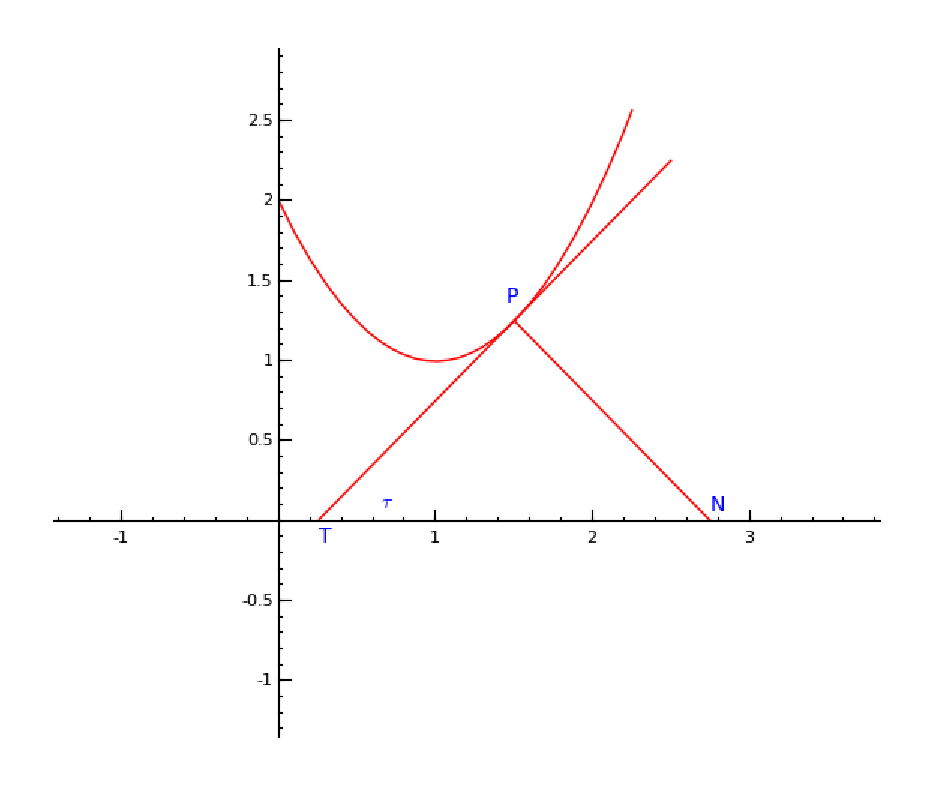
\includegraphics[height=4cm,width=6cm]{parabola-tangent2b.eps}
\end{center}
\end{minipage}
\caption{The tangent and normal line to a curve.}
\label{fig:tangent-line}
\end{figure}
%sage: p1 = plot(1+(x-1)^2, 0,2.25, rgbcolor=(1,0,0))
%sage: p2 = plot(x-1/4, 0.25, 2.5, rgbcolor=(1,0,0))
%sage: p3 = plot(-x+2.75, 1.5, 2.75, rgbcolor=(1,0,0))
%sage: t1 = text("$\\tau$", (0.7, 0.1))
%sage: t2 = text("P", (1.1, 1.1))
%sage: t3 = text("T", (0.3, -0.1))
%sage: t4 = text("N", (2.8, 0.1))
%sage: show(p1+p2+p3+t1+t2+t3+t4)

%\noindent
%(Caution: though $O$ and $T$ are drawn very close in this
%diagram, they are not the same point - $T$ is slightly to the 
%right of $O$.) %% new

\vskip .15in

If this line is tangent to the curve AB at the point 
$P_1(x_1,y_1)$, then from \S \ref{sec:64}, %§ 64, p. 73,

\[
   m = \tan \tau = \left [ \frac{dy}{dx} \right ]_{x=x_1, y=y_1} 
= \frac{dy}{dx}|_{x=x_1,y=y_1}.
\]
% new - removed the dy_1/dx_1 notation!!
Hence at point of contact $P_1(x_1,y_1)$ the equation of the 
{\it tangent line} 
(containing the segment %% new
$TP_1$
) %% new 
is

\begin{equation}
%(1) 
y - y_1 = (\frac{dy}{dx}|_{x=x_1,y=y_1})(x - x_1).
\label{eqn:1-65}
\end{equation}
\index{tangent line} 
The normal being perpendicular to tangent, its slope is

\[
-\frac{1}{m} 	= -\frac{dx}{dy} |_{x=x_1,y=y_1}	%By 55, p. 3 [§ 1]
\]
(item 55 in \S \ref{sec:1}).
And since it also passes through the point of contact 
$P_1(x_1,y_1)$, we have for the equation of the 
{\it normal line}
(containing the segment %% new
$P_1N$
) %% new

\begin{equation}
%(2) 
y - y_1 = -(\frac{dx}{dy}|_{x=x_1,y=y_1})(x - x_1).
\label{eqn:65-2}
\end{equation}
\index{normal line} 
That portion of the tangent which is % intercepted 
between $P_1(x_1,y_1)$ and the point of contact with %OX 
the $x$-axis %new
is called the 
{\it length of the tangent} ( = $TP_1$), and its projection on the %axis of X 
$x$-axis %new
is called the {\it length of the subtangent}\footnote{The subtangent 
is the segment obtained by projecting the portion $TP_1$ of the tangent line
onto the $x$-axis).} %%  new
(= $TM$). 
Similarly, we have the {\it length of the normal} ( = $P_1N$) 
and the {\it length of the subnormal} (= $MN$).
\index{length of the tangent}
\index{length of the subtangent}
\index{length of the normal}
\index{length of the subnormal}

In the triangle $TP_1M$, $\tan\, \tau = \frac{MP_1}{TM}$; 
therefore\footnote{If subtangent extends to the right of T, 
we consider it positive; if to the left, negative.}

\begin{equation}
%(3) 
TM = \frac{MP_1}{\tan \tau} = y_1 \frac{dx}{dy}|_{x=x_1,y=y_1} =
\ {\rm length\ of\ subtangent}.
\label{eqn:3-65}
\end{equation}
In the triangle $MP_1N$, $\tan\, \tau = \frac{MN}{MP_1}$; 
therefore\footnote{ If subnormal extends to the right of M, 
we consider it positive; if to the left, negative.}

\begin{equation}
%(4) 
MN =MP_1 \tan \tau = y_1 \frac{dy}{dx}|_{x=x_1,y=y_1} 
= {\rm \ length\ of\ subnormal}.
\label{eqn:4-65}
\end{equation}
The length of tangent ( $= TP_1$) and the length of normal 
( $= P_1N$) may then be found directly from Figure \ref{fig:tangent-line}, 
each being the hypotenuse of a right triangle having the two 
legs known. Thus

\begin{equation}
\begin{array}{ll}
TP_1 
&= \sqrt{\bar{TM}^2 + \bar{MP_1}^2}\\
&= \sqrt{ \left ( y_1 \frac{dx}{dy}|_{x=x_1,y=y_1} \right)^2 + (y_1)^2}\\
%(5) 
&= y_1 \sqrt{ \left ( \frac{dx}{dy}|_{x=x_1,y=y_1} \right)^2 + 1}\\
 &=
\ {\rm length\ of\ tangent}.
\end{array}
\label{eqn:5-65}
\end{equation}
Likewise,

\begin{equation}
\begin{array}{ll}
P_1N 
&= \sqrt{\bar{MN}^2 + \bar{MP_1}^2}\\
&= \sqrt{ \left ( \frac{dy}{dx}|_{x=x_1,y=y_1} \right)^2 + (y_1)^2}\\
%(6) 
&= y_1 \sqrt{ \left ( \frac{dy}{dx}|_{x=x_1,y=y_1} \right)^2 + 1}\\
 &=
\ {\rm length\ of\ normal}.
\end{array}
\label{eqn:6-65}
\end{equation}

The student is advised to get the lengths of the tangent 
and of the normal directly from the figure rather than by using %(5) and (6).
these equations.

When the length of subtangent or subnormal at a point on 
a curve is determined, the tangent and normal may be easily constructed.

\section{Exercises}

\begin{enumerate}

\item
%1
Find the equations of tangent and normal, lengths of subtangent, 
subnormal tangent, and normal at the point $(a,a)$ on the 
cissoid $y^2 = \frac{x^3}{2a - x}$.

\begin{figure}[h!]
%\begin{tabular}{cc}
\begin{minipage}{\textwidth}
\begin{center}
%\vspace{1.0 cm}
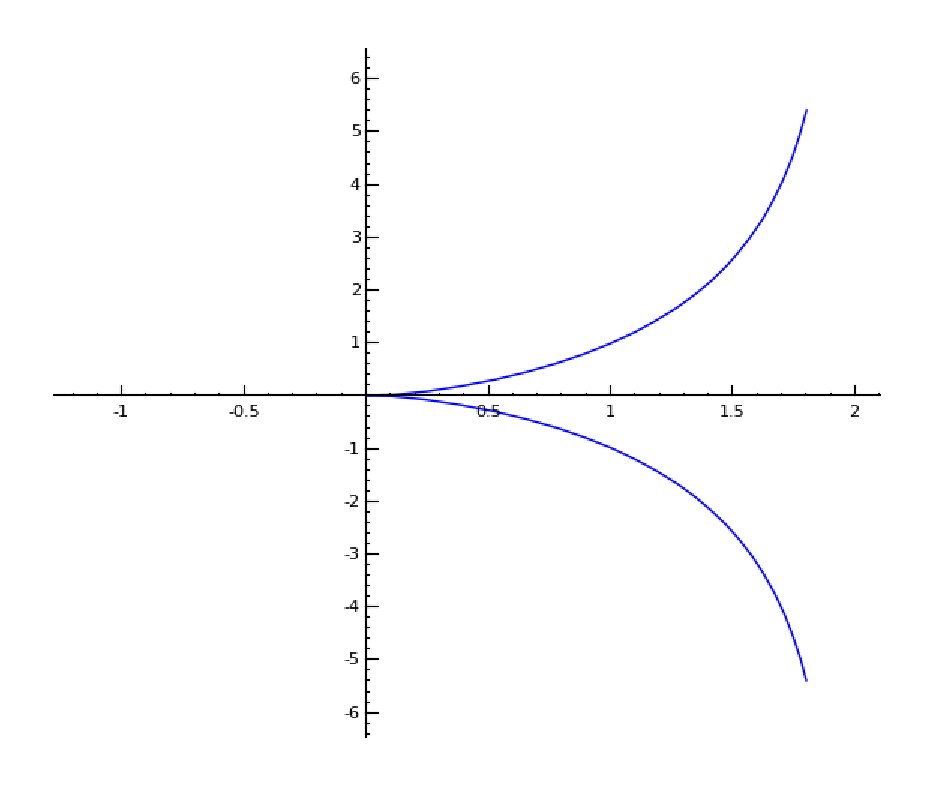
\includegraphics[height=5cm,width=5cm]{cissoid.eps}
\end{center}
\end{minipage}
\caption{Graph of cissoid $y^2 = \frac{x^3}{2a - x}$ with $a=1$.}
\label{fig:cissoid}
\end{figure}
%sage: p1 = plot(sqrt(x^3/(2-x)), 0,1.85, rgbcolor=(1,0,0))
%sage: p2 = plot(-sqrt(x^3/(2-x)), 0,1.85, rgbcolor=(1,0,0))
%sage: show(p1+p2)

Solution. 	
$\frac{dy}{dx} 	=\ \frac{3ax^2 - x^3}{y(2a - x)^2}$.
Hence 	

\[
\frac{dy_1}{dx_1} = \left [ \frac{dy}{dx} \right ]_{x = a, y = a} 	
=\ \frac{3a^3 - a^3}{a(2a - a)^2} = 2 
\]
is the slope of tangent. Substituting in (\ref{eqn:1-65}) 
gives
\[
  	y = 2x - a, 
\]
the equation of the tangent line.
Substituting in (\ref{eqn:65-2}) gives
\[
  	2y + x 	= 3a, 
\]
the equation of the normal line.
Substituting in (\ref{eqn:3-65}) gives

\[
TM 	= \frac{a}{2},
\]
the length of subtangent.
Substituting in (\ref{eqn:4-65}) gives

\[
  	MN 	= 2a,
\]
the length of subnormal.
Also 

\[
PT = \sqrt{(TM)^2 + (MP)^2} 
= \sqrt{\frac{a^2}{4} + a^2} 
= \frac{a}{2} \sqrt{5},
\]
which is the length of tangent,
and 

\[
PN = \sqrt{(MN)^2 + (MP)^2} 
= \sqrt{4a^2 + a^2} = a \sqrt{5},
\]
the length of normal.

\item
%2
Find equations of tangent and normal to the ellipse 
$x^2 + 2y^2 - 2xy - x = 0$ at the points where $x = 1$.

Ans. At $(1,0)$, $2y = x - 1$, $y + 2x = 2$.
At $(1,1)$, $2y = x + 1$, $y + 2x = 3$.

\item
%3
Find equations of tangent and normal, lengths of subtangent 
and subnormal at the point $(x_1,y_1)$ on the 
circle\footnote{In Exs. 3 and 5 the student should notice that 
if we drop the subscripts in equations of tangents, they 
reduce to the equations of the curves themselves.}
$x^2 + y^2 = r^2$.

Ans. $x_lx + y_1y = r^2$, $x_1y - y_1x = 0$, 
$-x_1, -\frac{{y_1}^2}{x_1}$.

\item
%4
Show that the subtangent to the parabola $y^2 = 4px$ is bisected 
at the vertex, and that the subnormal is constant and equal to $2p$.

\item
%5
Find the equation of the tangent at $(x_1,y_1)$ to the ellipse 
$\frac{x^2}{a^2} + \frac{y^2}{b^2} = 1$.

Ans. $\frac{x_1x}{a^2} + \frac{y_1y}{b^2} = 1$.

Here's how to find the length of tangent, normal, 
subtangent and subnormal of this in \sage 
using the values $a=1$, $b=2$
(so $x^2 + \frac{y^2}{4} = 1$) and $x_1=4/5$, $y_1=6/5$.

\vskip .1in

\begin{Verbatim}[fontsize=\small,fontfamily=courier,fontshape=tt,frame=single,label=\sage]

sage: x = var("x")
sage: y = var("y")
sage: F = x^2 + y^2/4 - 1
sage: Dx = -diff(F,y)/diff(F,x); Dx; Dx(4/5,6/5)
-y/(4*x)
-3/8
sage: Dy = -diff(F,x)/diff(F,y); Dy; Dy(4/5,6/5)
-4*x/y
-8/3

\end{Verbatim}
\vskip .1in

\noindent
(For this \sage calculation, we have used the fact that $F(x,y)=0$ implies
$F_x(x,y)+\frac{dy}{dx}F_y(x,y)=0$, where $y$ is regarded as a function of 
$x$.) Therefore, we have (using (\ref{eqn:3-65}))

\[
{\rm length\ of\ subtangent} = y_1 \frac{dx}{dy}|_{x=x_1,y=y_1} =
(6/5)(-3/8)=-9/20,
\]
(using (\ref{eqn:4-65}))
\[
{\rm \ length\ of\ subnormal}
 = y_1 \frac{dy}{dx}|_{x=x_1,y=y_1} = (6/5)(-8/3)=-16/5,
\]
(using (\ref{eqn:5-65}))
\[
\begin{array}{ll}
{\rm length\ of\ tangent}
=y_1 \sqrt{ \left ( \frac{dx}{dy}|_{x=x_1,y=y_1} \right)^2 + 1}
&= (6/5)\sqrt{1+\frac{9}{64}}\\
&=3\sqrt{73}/20
=1.2816...\ ,
\end{array}
\]
and (using (\ref{eqn:6-65}))
\[
\begin{array}{ll}
{\rm length\ of\ normal}
= y_1 \sqrt{ \left ( \frac{dy}{dx}|_{x=x_1,y=y_1} \right)^2 + 1}
&=(6/5)\sqrt{1+\frac{64}{9}}\\
&=2\sqrt{73}/5
=3.4176...\ .
\end{array}
\]
 

\item
%6
Find equations of tangent and normal to the  Witch of Agnesi 
$y = \frac{8a^3}{4a^2 + x^2}$ as at the point where $x = 2a$.

Ans. $x + 2y = 4a$, $y = 2x - 3a$.

\item
%7
Prove that at any point on the catenary 
$y = \frac{a}{2}(e^{\frac{x}{a}} + e^{-\frac{x}{a}})$ 
the lengths of subnormal and normal are 
$\frac{a}{4}(e^{\frac{2x}{a}} - e^{-\frac{2x}{a}})$ and 
$\frac{y^2}{a}$ respectively.
\index{curve! catenary}

\item
%8
Find equations of tangent and normal, lengths of subtangent 
and subnormal, to each of the following curves at the points indicated:

\[
\begin{array}{ll}
(a)\ \  y = x^3\ {\rm at}\ 
(\frac{1}{2}, \frac{1}{8}) & 	(e)\ \  y = 9-x^2 \ {\rm at}\ (-3,0)\\
 & \\
(b)\ \  y^2 = 4x \ {\rm at}\  (9,-6) & 	(f)\ \  x^2 = 6y \ {\rm where}\ x = -6\\
 & \\
(c)\ \  x^2 + 5y^2 = 14\ {\rm where}\  y = 1 &	(g)\ \  x^2 - xy + 2x - 9 = 0\ {\rm at}\ (3,2)\\
 & \\
(d)\ \  x^2 + y^2 = 25 at (-3,-4)  & (h)\ \  2x^2 - y^2 = 14\ {\rm at}\ (3,-2)
\end{array}
\]

\item
%9
Prove that the length of subtangent to $y = a^x$ is 
constant and equal to $\frac{1}{\log a}$.

\item
%10
Get the equation of tangent to the parabola 
$y^2 = 20x$ which makes an angle of 
$45^o=\pi/4$ with the %axis of X.
$x$-axis.

Ans. $y = x + 5$.
(Hint: First find point of contact by method of 
Example \ref{ex:64}.) %1, (d), p. 74 [§ 64]

\item
%11
Find equations of tangents to the circle $x^2 + y^2 = 52$ which 
are parallel to the line $2x + 3y = 6$.

Ans. $2x + 3y \pm 26 = 0$

\item
%12
Find equations of tangents to the hyperbola 
$4x^2 - 9y^2 + 36 = 0$ which are perpendicular to the line 
$2y + 5x = 10$.

Ans. $2x - 5y \pm 8 = 0$.

\item
%13
Show that in the equilateral hyperbola 
$2xy = a^2$ the area of the triangle formed by a tangent 
and the coordinate axes is constant and equal to $a^2$.

\item
%14
Find equations of tangents and normals to the curve 
$y^2 = 2x^2 - x^3$ at the points where $x = 1$.

Ans. At $(1,1)$, $2y = x + 1$, $y + 2x = 3$.
At $(1,-1)$, $2y =-x-1$, $y-2x = -3$.

\item
%15
Show that the sum of the intercepts of the tangent to the parabola
$x^{\frac{1}{2}} + y^{\frac{1}{2}} = a^{\frac{1}{2}}$.

\item
%16
Find the equation of tangent to the curve 
$x^2(x + y) = a^2(x-y)$ at the origin.

\item
%17
Show that for the hypocycloid 
$x^{\frac{2}{3}} + y^{\frac{2}{3}} = a^{\frac{2}{3}}$ that 
portion of the tangent included between the coordinate 
axes is constant and equal to $a$.
\index{hypocycloid}

\noindent
(This curve is parameterized by $x=a\cos(t)^3$, 
$y=a\sin(t)^3$, $0\leq t\leq 2\pi$. Parametric equations shall be 
discussed in the next section.)
 
\item
%18
Show that the curve $y = ae^{\frac{x}{c}}$ has a constant subtangent.

\end{enumerate}

%66. 
\section{Parametric equations of a curve}
\label{sec:66}

Let the equation of a curve be

\begin{equation}
%(A) 
F(x,y) = 0.
\label{eqn:A-66}
\end{equation}
If $x$ is given as a function of a third variable, $t$ say, 
called a {\it parameter}, then by virtue of (\ref{eqn:A-66}) 
$y$ is also a function of $t$, and the same functional 
relation (\ref{eqn:A-66}) between $x$ and $y$ may generally 
be expressed by means of equations in the form
\index{parameter}

\begin{equation}
%(B) 
\begin{cases} 
x = f(t), \\ 
y = g(t) 
\end{cases}
\label{eqn:B-66}
\end{equation}
each value of $t$ giving a value of $x$ and a value of $y$. 
Equations (\ref{eqn:B-66}) are called 
{\it parametric equations of the curve}. 
\index{parametric equations}
If we eliminate $t$ between equations (\ref{eqn:B-66}), 
it is evident that the relation (\ref{eqn:A-66}) must result. 

\begin{example}
{\rm
For example, take equation of circle

\[
x^2 + y^2= r^2\ {\rm or}\  y = \sqrt{r^2 - x^2}.
\]
%Let 	$x 	= r\cos\, t$, $y = r\sin\, t$, and 
We have

\begin{equation}
%(C) 	
\begin{cases} 
x= r\cos\, t \\ 
y  = r\sin\, t
\end{cases} 
\label{eqn:C-66}
\end{equation}	
as parametric equations of the circle, % in the figure, 
$t$ being the parameter\footnote{Parameterizations are not
unique. Another set of parametric 
equations of the first quadrant of the circle
is given by $x=\frac{\sqrt{2t}}{\sqrt{1+t^2}}$,
$y=\frac{1-t}{\sqrt{1+t^2}}$, for example%% new footnote
.}.

If we eliminate $t$ between equations (\ref{eqn:C-66}) 
by squaring and adding the results, we have

\[
 x^2 + y^2 = r^2(\cos^2t + \sin^2t) = r^2,
\]
the rectangular equation of the circle. 
It is evident that if $t$ varies from $0$ to $2\pi$, 
the point $P(x,y)$ will describe a complete circumference.
}
\end{example}

In \S \ref{sec:71} %§ 71 
we shall discuss the motion of a point $P$, which motion is 
defined by equations such as

\[
\begin{cases}
x = f(t), \\ 
y=g(t) 
\end{cases}
\]
We call these the {\it parametric equations of the path}, 
the time $t$ being the parameter. 
\index{parametric equations of the path}

\begin{example}
{\rm
%In Example 2, \S \ref{sec:examplesp93}, %p. 93, 
%we will see that
Newtonian physics tells us that %new

\[
\begin{cases} 
x = v_0 \cos \alpha \cdot t, \\ 
y = -\frac{1}{2} gt^2 + v_0 \sin \alpha \cdot t 
\end{cases}
\]
are really the parametric equations of the trajectory 
of a projectile\footnote{Subject to (downward) gravitational
force but no wind resistance or other external forces.}, %% new
the time $t$ being the parameter. The elimination of $t$ 
gives the rectangular equation of the trajectory

\[
  y = x \tan \alpha - \frac{gx^2}{2v_0^2 \cos^2 \alpha}.
\]

}
\end{example}

Since from (\ref{eqn:B-66}) $y$ is given as a function of $t$, 
and $t$ as a function of $x$, we have

\[
\begin{array}{ll}
\frac{dy}{dx} 
&	= \frac{dy}{dt} \cdot \frac{dt}{dx}
\ \ \ {\rm by\ XXV}\\
& 
= \frac{dy}{dt} \cdot \frac{1}{\frac{dx}{dt}}\ \ \ {\rm by\ XXVI}
\end{array}
\]
that is,

\begin{equation}
%(D) 	
\frac{dy}{dx} 	= \frac{\frac{dy}{dt}}{\frac{dx}{dt}} 
= \frac{g'(t)}{f'(t)}.
\label{eqn:D-66}
\end{equation}	
Hence, if the parametric equations of a curve are given, 
we can find equations of tangent and normal, lengths of 
subtangent and subnormal at a given point on the curve, by 
first finding the value of $\frac{dy}{dx}$ at that point 
from (\ref{eqn:D-66}) 
and then substituting in formulas (\ref{eqn:1-65}), (\ref{eqn:65-2}), 
(\ref{eqn:3-65}), (\ref{eqn:4-65}) of the last section.

\begin{example}
{\rm
Find equations of tangent and normal, lengths of subtangent 
and subnormal to the ellipse

\begin{equation}
%(E) 
\begin{cases} 
x = a \cos \phi, \\ 
y = b \sin \phi, 
\end{cases}
\label{eqn:E-66}
\end{equation}	
at the point where $\phi = \frac{\pi}{4}$.

As in Figure \ref{fig:ellipse} draw the major and minor auxiliary circles 
of the ellipse. Through two points B and C on the same 
radius draw lines parallel to the axes of coordinates. 
These lines will intersect in a point $P(x,y)$ on the ellipse, because
$x = OA = OB\cos\phi = a\cos\phi$
and $y = AP = OD = OC\sin\phi = b\sin\phi$,
or, $\frac{x}{a} = \cos \phi$ and 
$\frac{y}{b} = \sin \phi$.
Now squaring and adding, we get

\[
   \frac{x^2}{a^2} + \frac{y^2}{b^2} = \cos^2 \phi + \sin^2 \phi = 1,
\]
the rectangular equation of the ellipse. 
$\phi$ is sometimes called 
the {\it eccentric angle} of the ellipse at the point P.

\begin{figure}[h!]
%\begin{tabular}{cc}
\begin{minipage}{\textwidth}
\begin{center}
%\vspace{1.0 cm}
%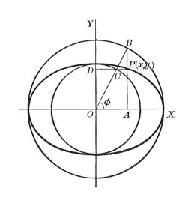
\includegraphics[height=4cm,width=4cm]{ellipse.eps}
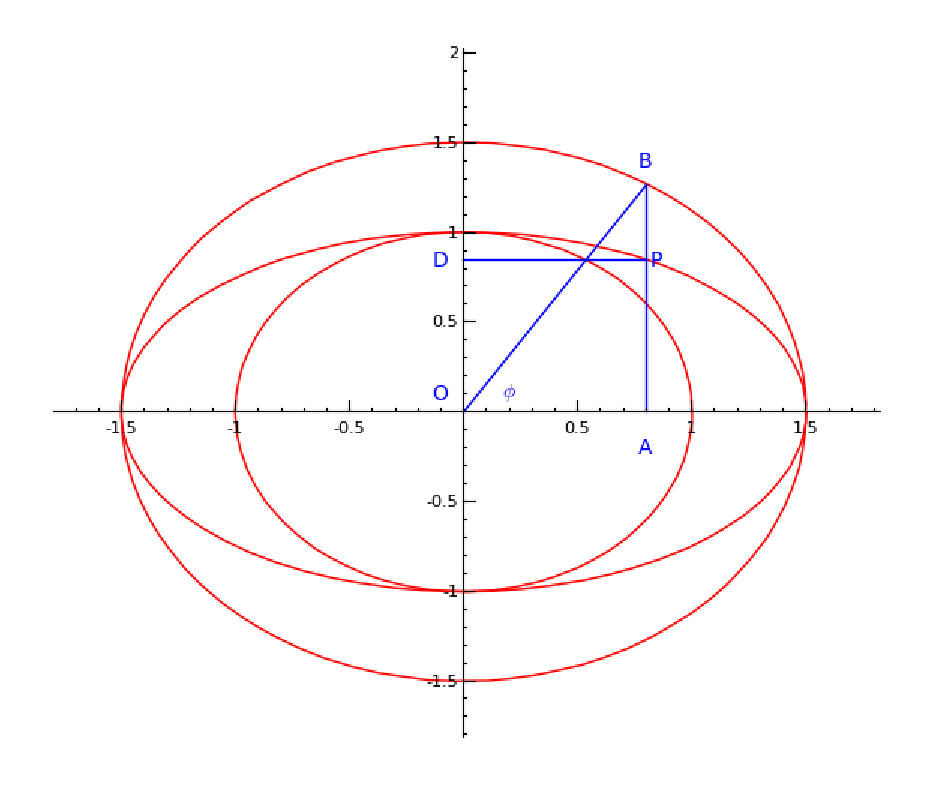
\includegraphics[height=6cm,width=6cm]{ellipse2.eps}
\end{center}
\end{minipage}
%\caption{Scan of Granville's graphic of an ellipse.}
\caption{Auxiliary circles of an ellipse.}
\label{fig:ellipse}
\end{figure}
%sage: p1 = parametric_plot([cos(t),sin(t)], 0, 2*pi, rgbcolor=(1,0,0))
%sage: p2 = parametric_plot([(3/2)*cos(t),sin(t)], 0, 2*pi, rgbcolor=(1,0,0))
%sage: p3 = parametric_plot([(3/2)*cos(t),(3/2)*sin(t)], 0, 2*pi, rgbcolor=(1,0,0))
%sage: p4 = line([(0.8,0),(0.8,1.265)])
%sage: p5 = line([(0,0),(0.8,1.265)])
%sage: p6 = line([(0,0.85),(0.8,0.85)])
%sage: t1 = text("A", (0.8,-0.2))
%sage: t2 = text("B", (0.8,1.4))
%sage: t3 = text("$\phi$", (0.2,0.1))
%sage: t4 = text("O", (-0.1,0.1))
%sage: t5 = text("D", (-0.1,0.85))
%sage: t6 = text("P", (0.85,0.85))
%sage: show(p1+p2+p3+p4+p5+p6+t1+t2+t3+t4+t5+t6)


Solution. 
The parameter being $\phi$, $\frac{dx}{d\phi} = - a \sin \phi$,
$\frac{dy}{d\phi} = b \cos \phi$.

Substituting $\phi = \frac{\pi}{4}$ in the given equations 
(\ref{eqn:E-66}), we get 
$\left ( \frac{a}{\sqrt{2}}, \frac{b}{\sqrt{2}} \right )$ 
as the point of contact. Hence
$\frac{dy}{dx}|_{x=x_1,y=y_1} = - \frac{b}{a}$.
Substituting in (\ref{eqn:1-65}), % (1), p76, 	

\[
y - \frac{b}{\sqrt{2}} = -\frac{b}{a} \left ( x - \frac{a}{\sqrt{2}} \right ),
\]
or, $bx + ay = \sqrt{2} ab$, the equation of tangent.
Substituting in (\ref{eqn:65-2}), %(2), p. 76, 	

\[
y - \frac{b}{\sqrt{2}} 	= \frac{a}{b} \left ( x - \frac{a}{\sqrt{2}} \right ),
\]
or, $\sqrt{2}(ax - by)=	a^2 - b^2$, the equation of normal.
Substituting in (\ref{eqn:3-65}) and (\ref{eqn:4-65}), %(3) and (4), p. 77,
we find

\[
\frac{b}{\sqrt{2}} \left ( -\frac{b}{a} \right ) 
= -\frac{b^2}{a\sqrt{2}}
,\]
the length of subnormal, and

\[
\frac{b}{\sqrt{2}} \left ( -\frac{a}{b} \right )
= -\frac{a}{\sqrt{2}},
\]
the length of subtangent.

}
\end{example}

\begin{example}
{\rm
Given equation of the cycloid in parametric form

\[
\begin{cases} 
x = a(\theta - \sin \theta), \\ 
y = a(1 - \cos \theta), 
\end{cases}
\]
$\theta$ being the variable parameter; 
find lengths of subtangent, subnormal, tangent, and 
normal at the point where $\theta = \frac{\pi}{2}$.

The path described by a point on the circumference of a circle 
which rolls without sliding on a fixed straight line is called 
the {\it cycloid}. 
\index{curve! cycloid}
Let the radius of the rolling circle be $a$, P the generating point, 
and M the point of contact with the fixed line OX, which is 
called {\it the base}. If arc PM equals OM in length, then 
P will touch at O if the circle is rolled to the left. 
We have, denoting angle POM by $\theta$,

\[
\begin{array}{ll}
  x &= OM - NM = a\theta - a\sin\theta = a(\theta- \sin\theta),\\  
    y &= PN = MC - AC = a - a\cos\theta = a(1 - \cos\theta),
\end{array}
\]
the parametric equations of the cycloid, the angle 
$\theta$ through which the rolling circle turns being 
the parameter. $OD = 2\pi a$ is called the {\it base of one arch} 
of the cycloid, and the point V is called the {\it vertex}. 
Eliminating $\theta$, we get the rectangular equation

\[
x = a \arccos \left ( \frac{a - y}{a} \right ) - \sqrt{ 2ay - y^2 }.
\]

\begin{figure}[h!]
%\begin{tabular}{cc}
\begin{minipage}{\textwidth}
\begin{center}
%\vspace{1.0 cm}
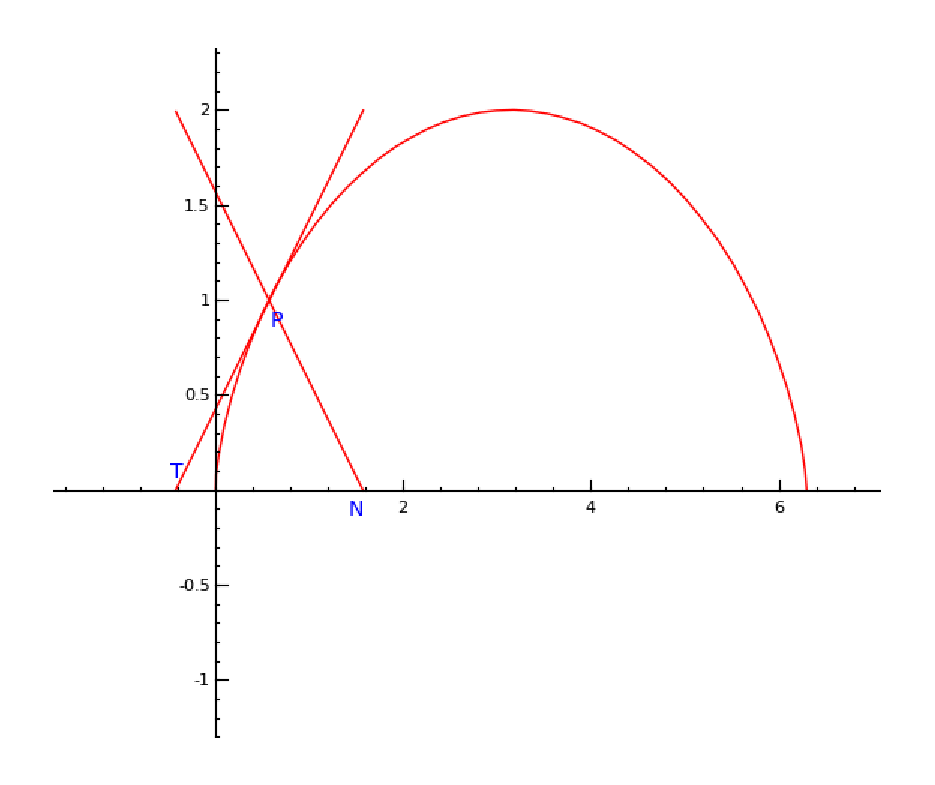
\includegraphics[height=4cm,width=8cm]{cycloid-tangent.eps}
\end{center}
\end{minipage}
\caption{Tangent line of a cycloid.}
\label{fig:cycloid}
\end{figure}
%sage: f1 = lambda t: [t-sin(t),1-cos(t)]
%sage: p1 = parametric_plot(f1(t), 0.0, 2*pi, rgbcolor=(1,0,0))
%sage: f2 = lambda t: [t+RR(pi)/2-1,t+1]
%sage: p2 = parametric_plot(f2(t), -1, 1, rgbcolor=(1,0,0))
%sage: t1 = text("P", (RR(pi)/2-1+0.1,1-0.1))
%sage: t2 = text("T", (-0.4,0.1))
%sage: show(p1+p2+t1+t2)

The \sage commands for creating this plot are as follows:

\vskip .1in

\begin{Verbatim}[fontsize=\small,fontfamily=courier,fontshape=tt,frame=single,label=\sage]

sage: t = var("t")
sage: f1 = lambda t: [t-sin(t),1-cos(t)]
sage: p1 = parametric_plot(f1(t), 0.0, 2*pi, rgbcolor=(1,0,0))
sage: f2 = lambda t: [t+RR(pi)/2-1,t+1]
sage: p2 = parametric_plot(f2(t), -1, 1, rgbcolor=(1,0,0))
sage: f3 = lambda t: [-t+RR(pi)/2,t]
sage: p3 = parametric_plot(f3(t), -1, 1, rgbcolor=(1,0,0))
sage: t1 = text("P", (RR(pi)/2-1+0.1,1-0.1))
sage: t2 = text("T", (-0.4,0.1))
sage: t3 = text("N", (RR(pi)/2,0))
sage: show(p1+p2+p3+t1+t2+t3)

\end{Verbatim}
\vskip .1in

\noindent
Solution:
\[
\frac{dx}{d\theta} 	
= a(1 - \cos \theta),\ \ \  \frac{dy}{d\theta} = a \sin \theta.
\]
Substituting in (\ref{eqn:D-66}), %(D) p. 80, 	

\[
\frac{dy}{dx} 	= \frac{\sin \theta}{1 - \cos \theta},
\]
the slope at any point.
Since $\theta = \frac{\pi}{2}$, the point of contact is 
$\left ( \frac{\pi a}{2} - a, a \right )$, and 
$\frac{dy}{dx}|_{x=x_1,y=y_1} = 1$.

Substituting in (\ref{eqn:3-65}), (\ref{eqn:4-65}), 
(\ref{eqn:5-65}), (\ref{eqn:6-65}) of the last section, 
we get

length of subtangent 	= $a$, 	

length of subnormal 	= $a$,

length of tangent 	= $a \sqrt{2}$, 

length of normal 	= $a \sqrt{2}$. 

}
\end{example}


\section{Exercises}

Find equations of tangent and normal, lengths of subtangent and 
subnormal to each of the following curves at the point indicated:

\begin{enumerate}

\item
%1
Curve:
$x = t^2$, $2y = t$; 

Point: 
$t = 1$.
 	
Tangent line: 
$x - 4y + 1 = 0$;

Normal line:
$8x + 2y - 9 = 0$;

Subtangent: 
$2$;

Subnormal: 
$\frac{1}{8}$.

\item
%2
Curve:
$x = t$, $y = t^3$;

Point: 
$t = 2$.

Tangent line: 
$12x - y - 16 = 0$;

Normal line:
$x + 12y - 98 = 0$;

Subtangent: 
$\frac{2}{3}$;

Subnormal: 
$96$.


\item
%3
Curve:
$x = t^2$, $y = t^3$;

Point: 
$t = 1$.

Tangent line: 
$3x - 2y - 1 = 0$;

Normal line:
$2x + 3y - 5 = 0$;

Subtangent: 
$\frac{2}{3}$;

Subnormal: 
$\frac{3}{2}$.

\item
%4
Curve:
$x = 2e^t$, $y = e^{- t}$; 

Point: 
$t = 0$.

Tangent line: 
$x + 2y - 4 = 0$;

Normal line:
$2x - y - 3 = 0$;

Subtangent: 
$-2$;

Subnormal: 
$-\frac{1}{2}$.

\item
%5
Curve:
$x = \sin\, t$, $y = \cos\, 2t$; 

Point: 
$t = \frac{\pi}{6}$. 	

Tangent line: 
$2y + 4x - 3 = 0$;

Normal line:
$4y - 2x - 1 = 0$;

Subtangent: 
$-\frac{1}{4}$;

Subnormal: 
$-1$.

\vskip .2in

\sage can help with the computations here:

\vskip .1in

\begin{Verbatim}[fontsize=\small,fontfamily=courier,fontshape=tt,frame=single,label=\sage]

sage: t = var("t")
sage: x = sin(t)
sage: y = cos(2*t)
sage: t0 = pi/6
sage: y_x = diff(y,t)/diff(x,t)
sage: y_x
-2*sin(2*t)/cos(t)
sage: y_x(t0)
-2
sage: m = y_x(t0); x0 = x(t0); y0 = y(t0)
sage: X,Y = var("X,Y")
sage: Y - y0 == m*(X - x0)
Y - 1/2 == -2*(X - 1/2)

\end{Verbatim}
\vskip .1in

\noindent
The last line is the point-slope form of the tangent 
line of the parametric curve at that point $t_0=\pi/6$
(so, $(x_0,y_0)=(\sin(t_0),\cos(2t_0))=( 1/2, 1/2)$).
We use $X$ and $Y$ in place of $x$ and $y$ so as to not 
over-ride the entries that \sage has stored for them.
Continuing the above \sage computations:

\vskip .1in

\begin{Verbatim}[fontsize=\small,fontfamily=courier,fontshape=tt,frame=single,label=\sage]

sage: x_y = diff(x,t)/diff(y,t)
sage: len_subtan = y(t0)*x_y(t0); len_subtan
-1/4
sage:
sage: len_subnor = y(t0)*y_x(t0); len_subnor
-1
sage: len_tan = y(t0)*sqrt(x_y(t0)^2+1); len_tan
sqrt(5)/4
sage: len_nor = y(t0)*sqrt(y_x(t0)^2+1); len_nor
sqrt(5)/2

\end{Verbatim}
\vskip .1in

\noindent
These tell us the length of the subtangent is $-\frac{1}{4}$
(as expected), as well as the lengths of the subnormal,
tangent and normal, using formulas
(\ref{eqn:D-66}), (\ref{eqn:3-65}), (\ref{eqn:4-65}), 
(\ref{eqn:5-65}), (\ref{eqn:6-65}) of the last section.

\item
%6
Curve:
$x = 1 - t$, $y = t^2$;

Point: 
$t = 3$.

\item
%7
Curve:
$x = 3t$; $y = 6t - t^2$;

Point:
$t = 0$.

\item
%8
Curve:
$x = t^3$; $y = t$;

Point:
$t = 2$.

\item
%9
Curve:
$x = t^3$, $y = t^2$;

Point:
$t = - 1$.

\item
%10
Curve:
$x = 2 - t$; $y = 3t^2$;

Point:
$t = 1$.

\item
%11
Curve:
$x = \cos\, t$, $y = \sin\, 2t$; 

Point:
$t = \frac{\pi}{3}$.

\item
%12
Curve:
$x = 3e^{-t}$, $y = 2e^t$;

Point:
$t = 0$.

\item
%13
Curve:
$x = \sin\, t$, $y = 2 \cos\, t$; 

Point:
$t = \frac{\pi}{4}$.

\item
%14
Curve:
$x = 4 \cos\, t$, $y = 3 \sin\, t$; 

Point:
$t = \frac{\pi}{2}$.

\item
%15
Curve:

Point:

\end{enumerate}

In the following curves find lengths of 
(a) subtangent, (b) subnormal, (c) tangent, (d) normal, at any point:

\begin{enumerate}
\addtocounter{enumi}{15}

\item
%16
The curve 	

\[
\begin{cases} 
x = a(\cos t + t \sin t), \\ 
y = a(\sin t - t \cos t). 
\end{cases}
\]

Ans. (a) $y\cot\, t$, (b) $y\tan\, t$, (c) $\frac{y}{\sin\, t}$, 
(d) $\frac{y}{\cos\, t}$.

\item
%17
The hypocycloid (astroid) 	

\[
\begin{cases} 
x = 4 a \cos^3 t, \\ 
y = 4a \sin^3 t. 
\end{cases}
\]

Ans. (a) $- y\cot\, t$, (b) $- y\tan\, t$, (c) $\frac{y}{\sin\, t}$, 
(d) $\frac{y}{\cos\, t}$.
\index{curve! hypocycloid (astroid)}

\item
%18
The circle 	

\[
\begin{cases} x = r \cos\, t, \\ 
y = r \sin\, t. 
\end{cases}
\]

\item
%19
The cardioid 	

\[
\begin{cases} 
x = a(2 \cos\, t - \cos\, 2t), \\ 
y = a(2 \sin\, t - \sin\, 2t). 
\end{cases}
\]
\index{curve! cardioid}

\item
%20
The folium 

\[
\begin{cases} 
x = \frac{3t}{1 + t^3} \\ 
y = \frac{3t^2}{1 + t^3}.
\end{cases}
\]
\index{curve! Folium of Descartes}

\item
%21
The hyperbolic spiral 	

\[
\begin{cases} 
x = \frac{a}{t} \cos\, t \\ 
y = \frac{a}{t} \sin\, t 
\end{cases}
\]
\index{curve! hyperbolic spiral}

\end{enumerate}

%67. 
\section{Angle between the radius vector and tangent}
\label{sec:67}

Angle between the radius vector drawn to a point on a curve 
and the tangent to the curve at that point. Let the equation of the 
curve in polar coordinates be $\rho = f(\theta)$.

Let P be any fixed point $(\rho,\theta)$ on the curve. If $\theta$, which we assume 
as the independent variable, takes on an increment $\Delta \theta$, then $\rho$ 
will take on a corresponding increment $\Delta \rho$. 

\begin{figure}[h!]
%\begin{tabular}{cc}
\begin{minipage}{\textwidth}
\begin{center}
%\vspace{1.0 cm}
%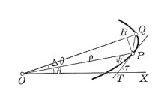
\includegraphics[height=2.5cm,width=3.5cm]{vector-angle.eps}
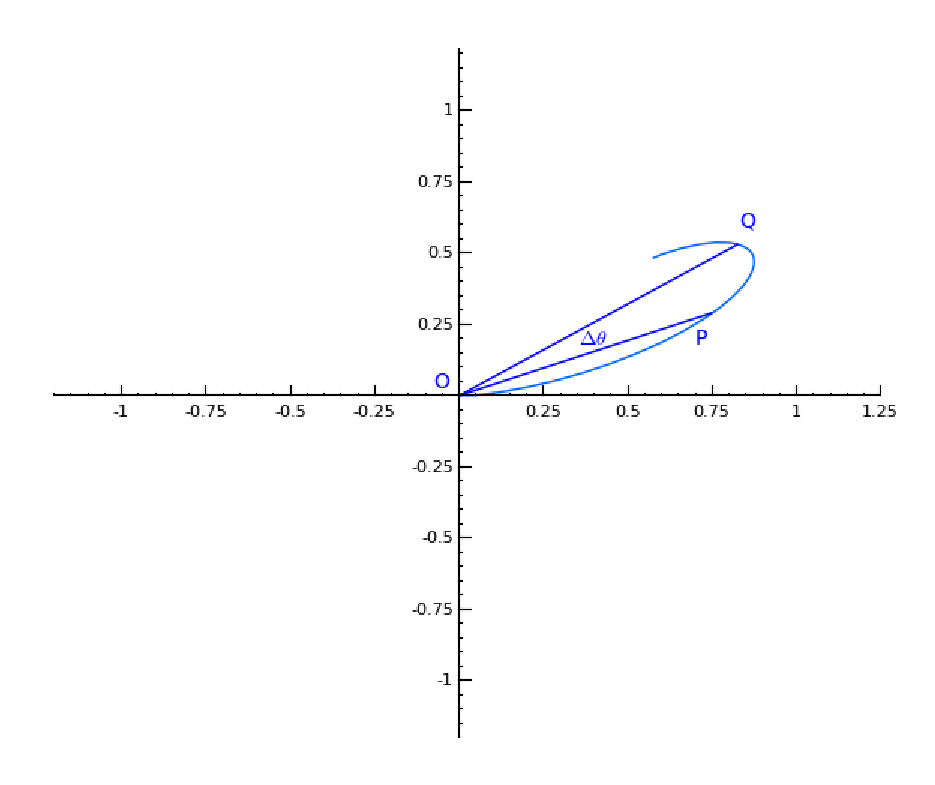
\includegraphics[height=6cm,width=9cm]{polar-tangent.eps}
\end{center}
\end{minipage}
\caption{Angle between the radius vector drawn to a point on a curve and the tangent to the curve at that point.}
\label{fig:vector-angle}
\end{figure}
%sage: xx = lambda r,t: r*cos(t)
%sage: yy = lambda r,t: r*sin(t)
%sage: r1 = lambda t: sin(3*t)^2
%sage: p1 = polar_plot(r1(t), 0, 2*pi/9, rgbcolor=hue(0.6))
%sage: t1 = text("P", (xx(r1(pi/10),pi/10)+0.1,yy(r1(pi/10),pi/10)))
%sage: t2 = text("Q", (xx(r1(pi/7),pi/7),yy(r1(pi/7),pi/7)+0.2))
%sage: p2 = line([(0,0),(xx(r1(pi/5.5),pi/5.5),yy(r1(pi/5.5),pi/5.5))])
%sage: p3 = line([(0,0),(xx(r1(pi/8.5),pi/8.5),yy(r1(pi/8.5),pi/8.5))])
%sage: t3 = text("$\Delta \\theta$", (0.4,0.2))
%sage: t4 = text("O", (-0.05,0.05))
%sage: show(p1+p2+p3+t1+t2+t3+t4)

Denote by Q the point 
$(\rho + \Delta \rho,\theta + \Delta \theta)$. Draw PR perpendicular to OQ. Then 
$OQ = \rho + \Delta \rho$, $PR = \rho \sin\Delta \theta$, and $OR = \rho \cos\Delta \theta$. 
Also,

\[
    \tan PQR = \frac{PR}{RQ} 
= \frac{PR}{OQ - OR} 
= \frac{\rho \sin \Delta \theta}{\rho + \Delta \rho - \rho \cos \Delta \theta}.
\]
Denote by $\psi$ the angle between the radius vector OP and the 
tangent PT. If we now let $\Delta \theta$ approach the limit zero, then

\begin{itemize}

\item[(a)] 
the point Q will approach indefinitely near P;

\item[(b)] 
the secant PQ will approach the tangent PT as a limiting position; and

\item[(c)] 
the angle PQR will approach $\psi$ as a limit.
\end{itemize}

Hence

\[
\tan\ \psi 	
=\ \lim_{\Delta \theta \to 0} \frac{\rho \Delta \theta}{\rho + \Delta \rho - \rho \cos \Delta \theta}
=\ \lim_{\Delta \theta \to 0} \frac{\rho \Delta \theta}{2 \rho \sin^2 \frac{\Delta \theta}{2} + \Delta \rho}
\]
(since, from 39, \S \ref{sec:1},
$\rho - \rho \cos \Delta \theta 
= \rho (1 - \cos \Delta \theta)= 2 \rho \sin^2 \frac{\Delta \theta}{2}$).
Dividing both numerator and denominator by $\Delta \theta$, this is
%equal to

\[
=\ \lim_{\Delta \theta \to 0} \frac{\frac{\rho \sin \Delta \theta}{\Delta \theta}}{\frac{2 \rho \sin^2 \frac{\Delta \theta}{2}}{\Delta \theta} + \frac{\Delta \rho}{\Delta \theta}}
=\ \lim_{\Delta \to 0} \frac{\rho \cdot \frac{\sin \Delta \theta}{\Delta \theta}}{\rho \sin \frac{\Delta \theta}{2} \cdot \frac{\sin \frac{\Delta \theta}{2}}{\frac{\Delta \theta}{2}} + \frac{\Delta \rho}{\Delta \theta}}.
\]
Since 

\[
\lim_{\Delta \theta \to 0} \left ( \frac{\Delta \rho}{\Delta \theta} \right ) 
= \frac{d\rho}{d\theta}\ {\rm and}\ \lim_{\Delta \theta \to 0} \left ( \sin \frac{\Delta \theta}{2} \right ) 
= 0,
\]
also 

\[
\lim_{\Delta \theta \to 0} \left ( \frac{\sin \Delta \theta}{\Delta \theta} \right ) = 1
\]
and 

\[
\lim_{\Delta \theta \to 0} \frac{\sin \frac{\Delta \theta}{2}}{\frac{\Delta \theta}{2}} = 1
\] 
by \S \ref{sec:22}, %§ 22, p. 21, 
we have

\begin{equation}
%(A) 
\tan\ \psi = \frac{\rho}{\frac{d\rho}{d\theta}}
\label{eqn:A-67}
\end{equation}	
From the triangle OPT we get

\begin{equation}
%(B) 
\tau = \theta + \psi.
\label{eqn:B-67}
\end{equation}	
Having found $\tau$, we may then find $\tan\,\tau$, the slope of the tangent 
to the curve at P. Or since, from (\ref{eqn:B-67}),

\[
    \tan \tau = \tan (\theta + \psi) = \frac{\tan \theta + \tan \psi}{1 - \tan \theta \tan \psi}
\]
we may calculate $\tan\, \psi$ from (\ref{eqn:A-67}) and substitute in the formula

\begin{equation}
%(C) 
{\rm slope\ of\ tangent}\ = \tan \tau = \frac{\tan \theta + \tan \psi}{1 - \tan \theta \tan \psi}.
\label{eqn:C-67}
\end{equation}	

\begin{example}
{\rm
Find $\psi$ and $\tau$ in the cardioid 
$\psi = a(1 -\cos\,\theta)$. Also find the slope at $\theta = \frac{\pi}{6}$.

Solution. $\frac{d\psi}{d\theta} = a \sin \theta$. 
Substituting in (\ref{eqn:A-67}) gives

\[
 \tan \psi 
= \frac{\rho}{\frac{d\rho}{d\theta}} 
= \frac{a(1 - \cos \theta)}{a \sin \theta} 
= \frac{2 a \sin^2 \frac{\theta}{2}}{2a \sin \frac{\theta}{2} \cos \frac{\theta}{2}} 
= \tan \frac{\theta}{2},
\]
by items 39 and 37, \S \ref{sec:1}. %39, p. 2,and 37, p.2
Since $\tan \psi = \tan \frac{\theta}{2}$, we have
$\psi = \frac{\theta}{2}$.

Substituting in (\ref{eqn:B-67}), 
$\tau = \theta + \frac{\theta}{2} = \frac{3\theta}{2}$.
so

\[
\tan\, \tau = \tan \frac{\pi}{4} = 1. 
\]
}
\end{example}

%\newpage

To find the angle of intersection $\phi$ of two curves $C$ and $C'$ whose 
equations are given in polar cooordinates, we may proceed as follows:

\begin{figure}[h!]
%\begin{tabular}{cc}
\begin{minipage}{\textwidth}
\begin{center}
%\vspace{1.0 cm}
%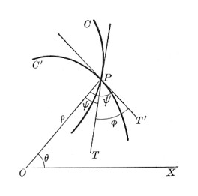
\includegraphics[height=2.5cm,width=3.5cm]{curves-angle.eps}
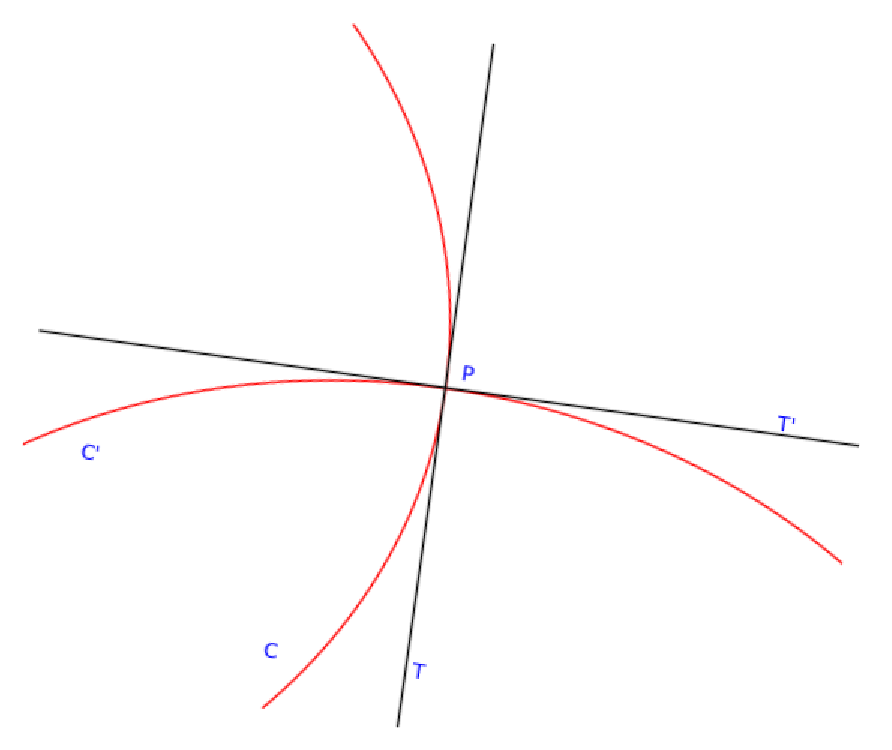
\includegraphics[height=5cm,width=8cm]{curves-intersect2.eps}
\end{center}
\end{minipage}
\caption{The angle between two curves.}
\label{fig:curves-angle}
\end{figure}
%sage: c1 = circle((1,0), 1, rgbcolor=(1,0,0))
%sage: c2 = circle((0,1), 1, rgbcolor=(1,0,0))
%sage: L1 = line([[1,0],[1,2]], rgbcolor=(0,0,0))
%sage: L2 = line([[0,1],[2,1]], rgbcolor=(0,0,0))
%sage: t1 = text("P", (1.03, 1.03))
%sage: t2 = text("T", (1.02, 0.5))
%sage: t3 = text("T\'", (1.5, 1.02))
%sage: t4 = text("C", (0.8, 0.5))
%sage: t5 = text("C\'", (0.5, 0.8))
%sage: show(c1+c2+L1+L2+t1+t2+t3+t4+t5, xmin = 1/2, xmax = 3/2, ymin = 1/2, ymax = 3/2, axes=False)

\begin{center}
angle TPT$'$ = angle OPT$'$ - angle OPT,
\end{center}
or, $\phi = \psi' - \psi$. Hence

\begin{equation}
%(D) 	
\ \tan\, \phi 	= \frac{\tan\, \psi' - \tan\, \psi}{1 + \tan\, \psi' \tan\, \psi},
\label{eqn:D-67}
\end{equation}	
where $\tan\, \psi'$ and $\tan\, \psi$ are calculated by (\ref{eqn:A-67}) 
from the two curves and evaluated for the point of intersection.

\begin{example}
{\rm
Find the angle of of intersection of the curves 
$\rho = a\sin\, 2\theta$, $\rho = a\cos\, 2\theta$.

Solution. Solving the two equations simultaneously, we get at the point of intersection

\[
 \tan\, 2\theta = 1, \,\ \ \ \  2\theta = 45^o=\pi/4,\ \ \  \theta = \frac{45}{2}^o=\pi/8.
\]
From the first curve, using (\ref{eqn:A-67}),

\[
    \tan \psi' = \frac{1}{2} \tan 2 \theta = \frac{1}{2}, 
\]
for $\theta = \frac{45}{2}^o=\pi/8$.
From the second curve,

\[
\tan \psi = -\frac{1}{2} \cot 2 \theta = -\frac{1}{2}, 
\]
for $\theta = \frac{45}{2}^o=\pi/8$.

Substituting in ((\ref{eqn:D-67}),

\[
   \tan \psi = \frac{ \frac{1}{2} + \frac{1}{2} }{ 1 - \frac{1}{4} } 
= \frac{4}{3}. 
\]
therefore $\psi = \arctan \frac{4}{3}$. 
}
\end{example}


%68. 
\section{Lengths of polar subtangent and polar subnormal}

Draw a line NT through the origin perpendicular to the 
radius vector of the point P on the curve. If PT is the 
tangent and PN the normal to the curve at P, 
then\footnote{When $\theta$ increases with $\rho$, $\frac{d\theta}{d\rho}$ 
is positive and $\rho$ is an acute angle, as in Figure \ref{fig:polar-subtangent}. 
Then the subtangent OT is positive and is measured to the right 
of an observer placed at O and looking along OP. When 
$\frac{d\theta}{d\rho}$ is negative, the subtangent is negative and 
is measured to the left of the observer.}

\begin{figure}[h!]
%\begin{tabular}{cc}
\begin{minipage}{\textwidth}
\begin{center}
%\vspace{1.0 cm}
%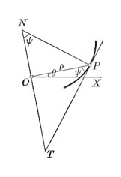
\includegraphics[height=3.5cm,width=2.5cm]{polar-subtangent.eps}
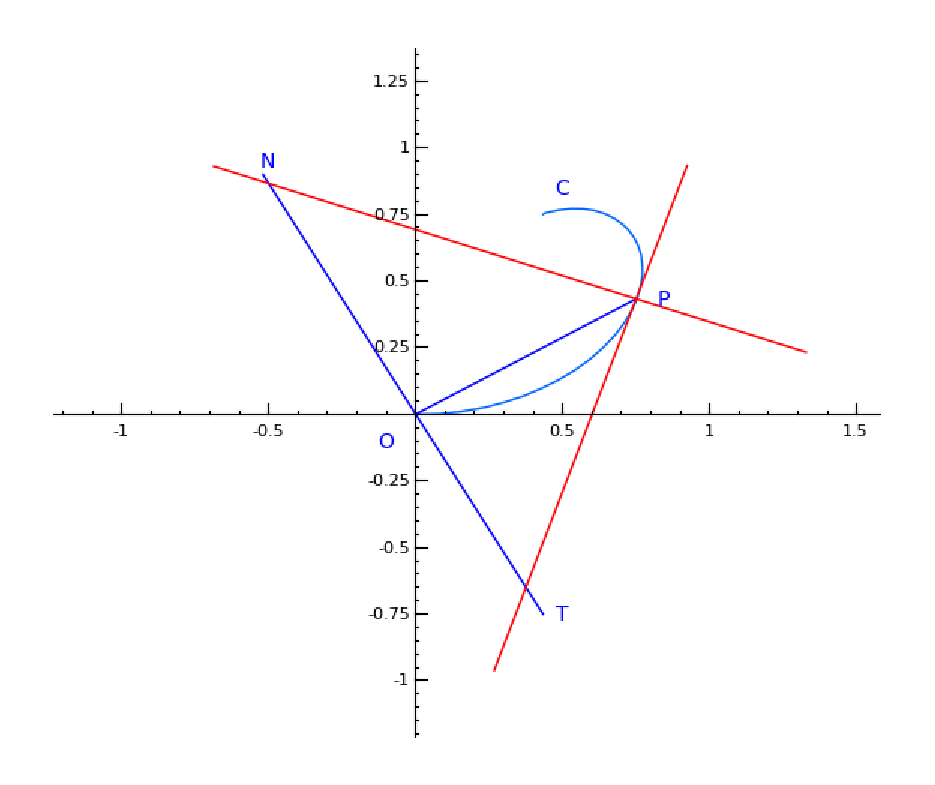
\includegraphics[height=6cm,width=6cm]{polar-subtangent2.eps}
\end{center}
\end{minipage}
%\caption{Scan of Granville's graphic of the polar subtangent and polar subnormal.}
\caption{The polar subtangent and polar subnormal.}
\label{fig:polar-subtangent}
\end{figure}

\begin{center}
OT = length of polar subtangent,
\end{center}
and 	
\begin{center}
ON = length of polar subnormal
\end{center}
of the curve at P.

In the triangle OPT, $\tan\, \psi = \frac{OT}{\rho}$. Therefore

\begin{equation}
%(7) 
OT = \rho \tan \psi = \rho^2 \frac{d\theta}{d\rho} 
=\ {\rm length\ of\ polar\ subtangent}.
\label{eqn:7-68}
\end{equation}	
In the triangle OPN, $\tan \psi = \frac{\rho}{ON}$. Therefore

\begin{equation}
%(8) 
ON = \frac{\rho}{\tan \psi} = \frac{d\rho}{d\theta} 
=\ {\rm length\ of\ polar\ subnormal}.
\label{eqn:8-68}
\end{equation}
The length of the polar tangent (= PT) and the length of the polar 
normal (= PN) may be found from the figure, each being the hypotenuse 
of a right triangle.

\begin{example}
{\rm
 Find lengths of polar subtangent and subnormal to the lemniscate 
$\rho^2 = a^2\cos\, 2\theta$.
\index{curve! lemniscate}

Solution. Differentiating the equation of the curve as an implicit 
function with respect to $\theta$,
or, 
$2 \rho \frac{d\rho}{d\theta} 	=\ - 2 a^2 \sin 2 \theta$,
$\frac{d\rho}{d\theta} 	=\ -\frac{a^2 \sin 2\theta}{\rho}$.

Substituting in (\ref{eqn:7-68}) and (\ref{eqn:8-68}), we get

\begin{center}
length of polar subtangent 	= $- \frac{\rho^3}{a^2 \sin 2\theta}$,
\\
length of polar subnormal 	= $- \frac{a^2 \sin 2\theta}{\rho}$.
\end{center}
If we wish to express the results in terms of $\theta$, find $\rho$ in
terms of $\theta$ from the given equation and substitute. 
Thus, in the above, $\rho = \pm a \sqrt{\cos 2 \theta}$; therefore 

\begin{center}
length of polar subtangent = $\pm a \cot 2 \theta \sqrt{\cos 2 \theta}$.
\end{center}

}
\end{example}

\section{Examples}

\begin{enumerate}
\item
%1
In the circle $\rho  = r\sin\, \theta$, find $\psi$ and $\tau$ in terms of 
$\theta$. 

Solution: $\psi = \theta$, $\tau=2\theta$.

\item
%2
In the parabola $\rho = a \sec^ \frac{\theta}{2}$, show that 
$\tau + \psi = \pi$.

\item
%3
In the curve $\rho^2 = a^2\cos\,2\theta$, show that $2\psi = \pi + 4\theta$.

\item
%4
Show that $\psi$ is constant in the logarithmic spiral 
$\rho  = e^{a\theta}$. Since the tangent makes a constant angle 
with the radius vector, this curve is also called the equiangular spiral.

\item
%5
Given the curve $\rho = a \sin^3 \frac{\theta}{3}$, prove that 
$\tau  = 4\psi$.

\vskip .2in

\sage can help with this problem. Using (\ref{eqn:A-67}) but with $t$ in place of
$\theta$ for typographical simplicity, we have

\vskip .15in

\begin{Verbatim}[fontsize=\small,fontfamily=courier,fontshape=tt,frame=single,label=\sage]

sage: a,t = var("a,t")
sage: r = a*sin(t/3)^3
sage: tanpsi = r/diff(r,t); tanpsi
sin(t/3)/cos(t/3)

\end{Verbatim}
\vskip .1in
\noindent
Therefore, $\tan(\psi) = \tan(\theta/3)$, so $\theta=3\psi$.
Therefore, according to (\ref{eqn:B-67}), we have 
$\tau=\theta+\psi=3\psi+\psi=4\psi$, as expected.


\item
%6
Show that $\tan\, \psi = \theta$ in the spiral of Archimedes 
$\rho  = a\theta$. Find values of $\psi$ when 
$\theta = 2\pi$ and $4\pi$. 

Solution: $\psi = 80^o 57' = 1.4128...$ and $85^o 27'=1.4913...$.

\item
%7
Find the angle between the straight line $\rho\cos\,\theta = 2a$ 
and the circle $\rho = 5a\sin\,\theta$. 

Solution: $\arctan \frac{3}{4}$.

\item
%8
Show that the parabolas $\rho = a \sec^2 \frac{\theta}{2}$ and 
$\rho = b \csc^2 \frac{\theta}{2}$ intersect at right angles.

\item
%9
Find the angle of intersection of $\rho = a\sin\,\theta$ and 
$\rho = a\sin\, 2\theta$. 

Solution: At origin $0^o$; at two other points $\arctan 3 \sqrt{3}$.

\item
%10
Find the slopes of the following curves at the points designated:

\begin{tabular}{lcc}
curve & point & solution (if given)\\ \hline
 & & \\
(a)\ \ $\rho = a(l - \cos,\theta)$ & $\theta = \frac{\pi}{2}$ & $-1$\\
(b)\ \  $\rho = a\sec^2 \theta$    & $\rho = 2a$              & $3$\\
(c)\ \ $\rho = a\sin\, 4\theta$    & origin                   &	$0, 1, \infty, -1$\\
(d)\ \ $\rho^2 = a^2\sin\, 4\theta$    & origin               &	$0, 1, \infty, -1$\\
(e)\ \ $\rho = a\sin\, 3\theta$    & origin                   & $0, \sqrt{3}, -\sqrt{3}$\\
(f)\ \ $\rho = a\cos\, 3\theta$    & 	origin & \\
(g) \ \ $\rho = a\cos\, 2\theta$    & origin & \\
(h)\ \ $\rho = a\sin\, 2\theta$    & $\theta = \frac{\pi}{4}$ & \\
(i)\ \ $\rho = a\sin\, 3\theta$    & $\theta = \frac{pi}{6}$ & \\
(j)\ \ $\rho = a\theta$           & $\theta = \frac{\pi}{2}$ & \\
(k)\ \ $\rho\theta = a$           & $\theta = \frac{\pi}{2}$ & \\
(l)\ \ $\rho = e^\theta$           & $\theta =  0$ & \\
\end{tabular}

\item
%11
Prove that the spiral of Archimedes $\rho  = a\theta$, and the reciprocal 
spiral $\rho = \frac{a}{\theta}$, intersect at right angles.
\index{curve! spiral of Archimedes}

\item
%12
Find the angle between the parabola $\rho = a sec^2 \frac{\theta}{2}$ and 
the straight line $\rho\sin\, \theta = 2a$. 

Solution: $45^o = \pi/4$.

\item
%13
Show that the two cardioids $\rho = a(1 + \cos\, \theta)$ and 
$\rho = a(1 - \cos\, \theta)$ cut each other perpendicularly.
\index{curve! cardioid}

\item
%14
Find lengths of subtangent, subnormal, tangent, and normal of 
the spiral of Archimedes $\rho  = a\theta$.
\index{curve! spiral of Archimedes}

Solution:
subt. = $\frac{\rho^2}{a}$, tan. = $\frac{\rho}{a} \sqrt{a^2 + \rho^2}$,
subn. = $a$, nor. = $\sqrt{a^2 + \rho^2}$.
The student should note the fact that the subnormal is constant.

\item
%15
Get lengths of subtangent, subnormal, tangent, and normal 
in the logarithmic spiral $\rho  = a^\theta$.
\index{curve! logarithmic spiral}

Solution:
subt. = $\frac{\rho}{\log a}$, 	
tan. = $\rho \sqrt{1 + \frac{1}{\log^2 a}}$,
subn. = $\rho\log\, a$,
nor. = $\rho \sqrt{1 + \log^2 a}$.

When $a = e$, we notice that subt. = subn., and tan. = nor.

\item
%16
Find the angles between the curves $\rho = a(1 + \cos\, \theta)$ and 
$\rho = b(1 - \cos\, \theta)$.

Solution: $0$ and $\frac{\pi}{2}$.

\item
%17
Show that the reciprocal spiral $\rho = \frac{a}{\theta}$ has a 
constant subtangent.

\item
%18
Show that the equilateral hyperbolas 
$\rho^2\sin\, 2\theta=a^2$, $\rho^2\cos\, 2\theta=b^2$
intersect at right angles.

\end{enumerate}

%69. 
\section{Solution of equations having multiple roots}

Any root which occurs more than once in an equation is 
called a {\it multiple root}. Thus $3$, $3$, $3$, $-2$ are the roots of

\[
%(A) 
x^4 - 7x^3 + 9x^2 + 27x - 54 = 0;
\]
hence $3$ is a multiple root occurring three times.
\index{multiple root}
Evidently this equation may also be written in the form
\[
    (x - 3)^3(x + 2) = 0.
\]

Let $f(x)$ denote an integral rational function of $x$ having 
a multiple root $a$, and suppose it occurs $m$ times. Then we may write

\begin{equation}	
%(B) 
f(x) = (x-a)^m\phi (x),
\label{eqn:B-69}
\end{equation}	
where $\phi (x)$ is the product of the factors corresponding to all 
the roots of $f(x)$ differing from $a$. Differentiating (\ref{eqn:B-69}),

\[
  f'(x) = (x-a)^m\phi '(x) + m\phi (x)(x - a)^{m - 1},
\]
or,

\begin{equation}	
%(C) 
f'(x) = (x-a)^{m - 1}[(x - a)\phi '(x) + m\phi (x)].
\label{eqn:C-69}
\end{equation}
Therefore $f'(x)$ contains the factor $(x - a)$ repeated $m - 1$ 
times and no more; that is, the {\it highest common factor} (H.C.F.) 
of $f(x)$ and $f'(x)$ has $m - 1$ roots equal to $a$.
\index{highest common factor}

In case $f(x)$ has a second multiple root $\beta$ occurring $r$ times, 
it is evident that the H.C.F. would also contain the factor 
$(x -\beta)^{r - 1}$ and so on for any number of different 
multiple roots, each occurring once more in $f(x)$ than in the H.C.F.

We may then state a {\it rule for finding the multiple roots} 
of an equation $f(x) = 0$ as follows:

\begin{itemize}
\item
FIRST STEP. Find $f'(x)$.

\item
SECOND STEP. Find the H.C.F. of $f(x)$ and $f'(x)$.

\item
THIRD STEP. Find the roots of the H.C.F. Each different 
root of the H.C.F. will occur once more in $f(x)$ than it does in the H.C.F.
\end{itemize}
If it turns out that the H.C.F. does not involve $x$, then $f(x)$ 
has no multiple roots and the above process is of no assistance 
in the solution of the equation, but it may be of interest to know 
that the equation has no equal, i.e. multiple, roots.


\begin{example}
{\rm
Solve the equation $x^3 - 8x^2 + 13x - 6 = 0$.

Solution. Place 	$f(x) = x^3 - 8x^2 + 13x - 6$.

First step. $f'(x) 	= 3x^2 - 16x + 13$.

Second step. 	H.C.F. 	= $x - 1$.

Third step. $x - 1 = 0$, therefore $x = 1$.

Since 1 occurs once as a root in the H.C.F., it will occur twice 
in the given equation; that is, $(x - 1)^2$ will occur there as 
a factor. Dividing $x^3 - 8x^2 + 13x - 6$ by $(x - 1)^2$ gives the 
only remaining factor $(x - 6)$, yielding the root $6$. The roots 
of our equation are then $1$, $1$, $6$. Drawing the graph of the function, 
we see that at the double root $x = 1$ the graph touches the $x$-axis
but does not cross it.

Note: Since the first derivative vanishes 
for every multiple root, it follows that the $x$-axis is tangent 
to the graph at all points corresponding to multiple roots. If a 
multiple root occurs an even number of times, the graph will not 
cross the $x$-axis at such a point (see Figure \ref{fig:multiple-roots}); 
if it occurs an odd number of times, the graph will cross.

\begin{figure}[h!]
%\begin{tabular}{cc}
\begin{minipage}{\textwidth}
\begin{center}
%\vspace{1.0 cm}
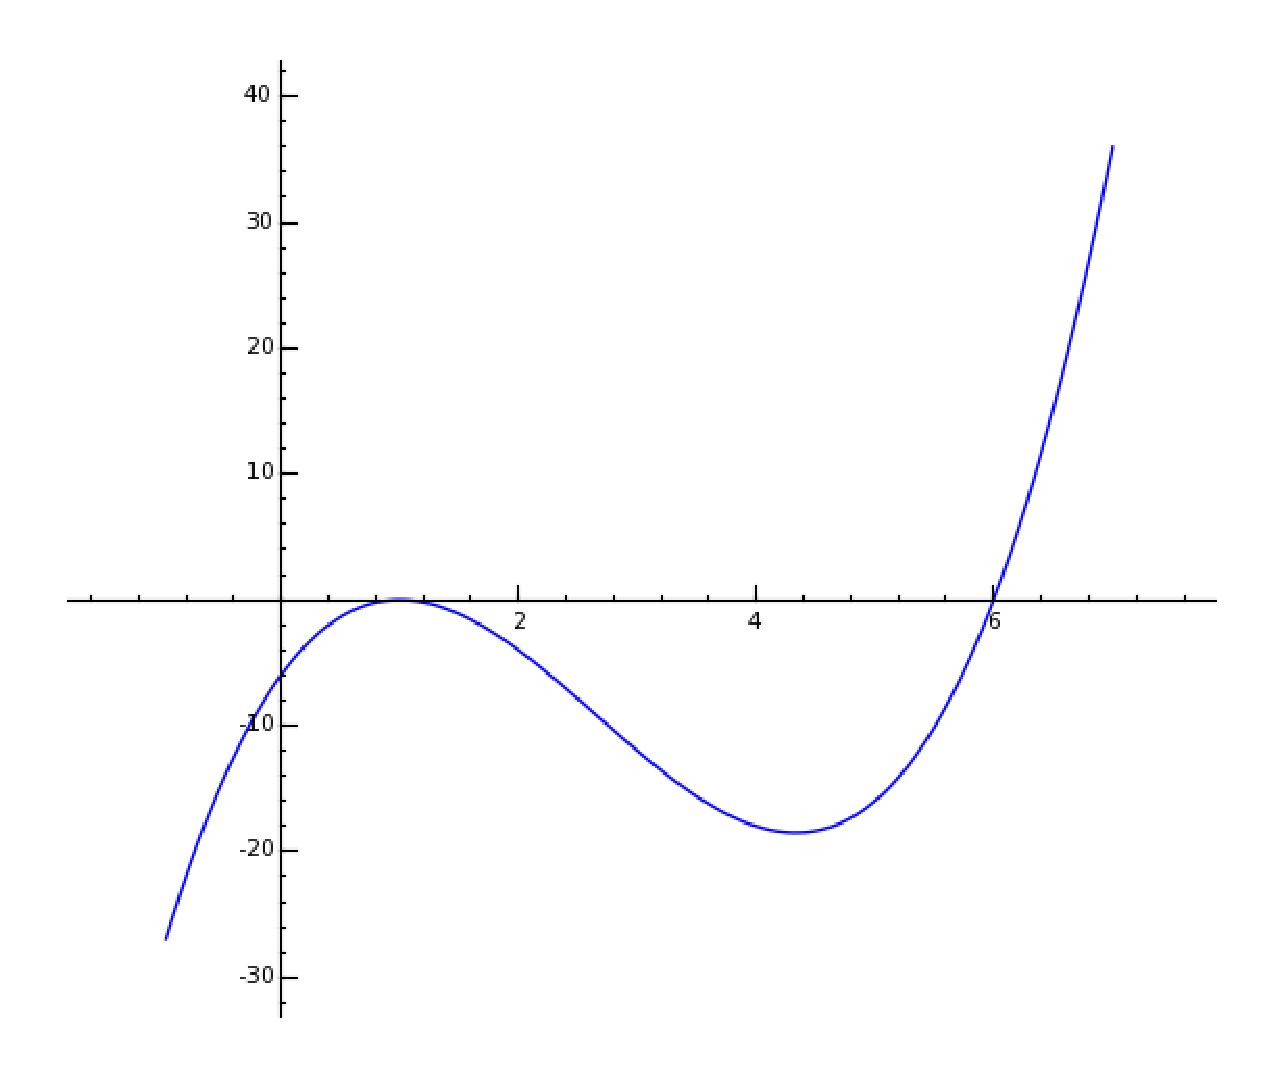
\includegraphics[height=2.5cm,width=3.5cm]{multiple-roots.eps}
\end{center}
\end{minipage}
\caption{plot of $f(x) = (x-1)^2(x-6)$ illustrating a multiple root.}
\label{fig:multiple-roots}
\end{figure}
%sage: P = plot((x-6)*(x-1)^2,-1,7)
%sage: show(P)



}
\end{example}


\section{Examples}

\begin{enumerate}
\item
%1
$x^3 - 7x^2 + 16x - 12 = 0$. 	

Ans. 	$2$, $2$, $3$.

\item
%2
$x^4 - 6x^2 - 8x - 3 = 0$.

\item
%3
$x^4 - 7x^3 + 9x^2 + 27x - 64 = 0$. 

Ans. $3$, $3$, $3$, $-2$.

\item
%4
$x^4 - 5x^3 - 9x^2 + 81x - 108 = 0$. 	  	

Ans. $3$, $3$, $3$, $-4$.

\item
%5
$x^4 + 6x^3 + x^2 - 24x + 16 = 0$. 

Ans. $1$, $1$, $-4$, $-4$.

\item
%6
$x^4 - 9x^3 + 23x^2 - 3x - 36 = 0$. 

Ans. $3$, $3$, $-1$, $4$.

\item
%7
$x^4 - 6x^3 + 10x^2 - 8 = 0$. 

Ans. $2$, $2$, $1 \pm \sqrt{3}$.

\vskip .2in

\sage can help with this problem. 

\vskip .15in

\begin{Verbatim}[fontsize=\small,fontfamily=courier,fontshape=tt,frame=single,label=\sage]

sage: x = var("x")
sage: solve(x^4 - 6*x^3 + 10*x^2 - 8 == 0,x)
[x == 1 - sqrt(3), x == sqrt(3) + 1, x == 2]
sage: factor(x^4 - 6*x^3 + 10*x^2 - 8)
(x - 2)^2*(x^2 - 2*x - 2)

\end{Verbatim}
\vskip .1in
\noindent
This tells use that the root $2$ occurs with multiplicity $2$.

\item
%8
$x^5 - x^4 - 5x^3 + x^2 + 8x + 4 = 0$.

\vskip .2in

\sage can help with this problem. 

\vskip .15in

\begin{Verbatim}[fontsize=\small,fontfamily=courier,fontshape=tt,frame=single,label=\sage]

sage: x = var("x")
sage: solve(x^5 - 15*x^3 + 10*x^2 + 60*x - 72 == 0,x)
[x == -3, x == 2]
sage: factor(x^5 - 15*x^3 + 10*x^2 + 60*x - 72)
(x - 2)^3*(x + 3)^2

\end{Verbatim}
\vskip .1in
\noindent
This tells use that the root $2$ occurs with multiplicity $3$ amd
the root $-3$ occurs with multiplicity $2$, as expected.



\item
%9
$x^5 - 15x^3 + 10x^2 + 60x - 72 = 0$. 

Ans. $2$, $2$, $2$, $-3$, $-3$.

\item
%10
$x^5 - 3x^4 - 5x^3 + 13x^2 + 24x + l0 = 0$. 	 

\end{enumerate}

Show that the following four equations have no multiple (equal) roots:

\begin{enumerate}
\addtocounter{enumi}{10}

\item
%11
$x^3 + 9x^2 + 2x - 48 = 0$.

\item
%12
$x^4 - 15x^2 - 10x + 24 = 0$.

\item
%13
$x^4 - 3x^3 - 6x^2 + 14x + 12 = 0$.

\item
%14
$x^n - a^n = 0$.

\item
%15
Show that the condition that the equation

\[
 x^3 + 3qx + r = 0
\]
shall have a double root is $4q^3 + r^2 = 0$.

\item
%16
Show that the condition that the equation

\[
   x^3 + 3px^2 + r = 0
\]
shall have a double root is $r(4p^3 + r) = 0$.

\end{enumerate}


%70. 
\section{Applications of the derivative in mechanics}

Included also are applications to velocity and rectilinear motion. 

Consider the motion of a point P on the straight line AB.


\begin{figure}[h!]
%\begin{tabular}{cc}
\begin{minipage}{\textwidth}
\begin{center}
%\vspace{1.0 cm}
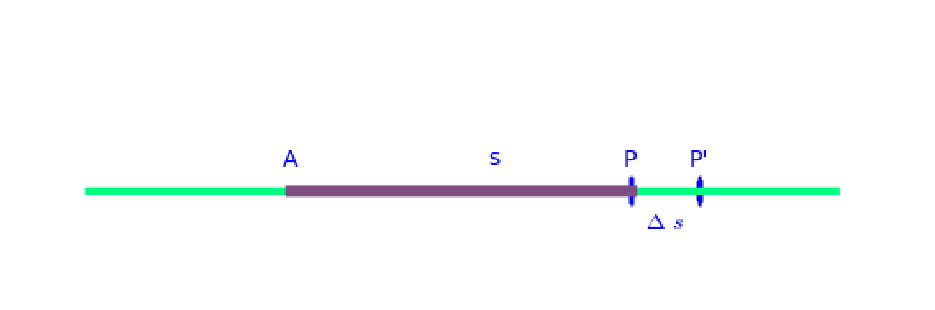
\includegraphics[height=2cm,width=8cm]{linear-motion2.eps}
\end{center}
\end{minipage}
\caption{Scan of Granville's graphic of the rectilinear motion.}
\label{fig:linear-motion}
\end{figure}
%sage: f = lambda x: 0
%sage: G1 = plot(f, -5, 6, thickness=3, rgbcolor=(0.0,1,0.5))
%sage: G2 = plot(f, -2, 3, thickness=5, rgbcolor=(0.5,0.3,0.5))
%sage: t1 = text("A", (-2,0.1))
%sage: t2 = text("P", (3,0.1))
%sage: t3 = text("P\'", (4.0,0.1))
%sage: t4 = text("$\Delta\, s$", (3.5,-0.1))
%sage: t5 = text("s", (1,0.1))
%sage: p1 = disk((3.0, 0.0), 0.05, (0, 2*pi))
%sage: p2 = disk((4.0, 0.0), 0.05, (0, 2*pi))
%sage: show(G1+G2+t1+t2+t3+t4+t5+p1+p2, axes=False)

Let $s$ be the distance measured from some fixed point as A to any 
position of P, and let $t$ be the corresponding elapsed time. 
To each value of $t$ corresponds a position of P and 
therefore a distance (or space) $s$. Hence $s$ will be a 
function of $t$, and we may write

\[
s = f(t)
\]
Now let $t$ take on an increment $\Delta t$; then $s$ takes on an 
increment\footnote{Δs being the space or distance passed 
over in the time $\Delta t$.} $\Delta s$, and

\begin{equation}
%(A) 
\frac{\Delta s}{\Delta t} = {\rm the\ average\ velocity}
\label{eqn:A-70}
\end{equation}	
of P during the time interval $\Delta t$. If P moves with uniform 
motion, the above ratio will have the same value for every 
interval of time and is the velocity at any instant.

For the general case of any kind of motion, uniform 
or not, we define the {\it velocity} (or, time rate of change of s) 
at any instant as the limit of the ratio $\frac{\Delta s}{\Delta t}$ as 
$\Delta t$ approaches the limit zero; that is, 
\index{velocity}

\[
  	v = \lim_{\Delta t \to 0} \frac{\Delta s}{\Delta t},
\]
or

\begin{equation}
%(9) 	
v = \frac{ds}{dt}
\label{eqn:9-70}
\end{equation}	
{\it The velocity is the derivative of the distance (= space) with respect to the time.}

To show that this agrees with the conception we already have 
of velocity, let us find the velocity of a falling body at the end of two seconds.

By experiment it has been found that a body falling freely from 
rest in a vacuum near the earth's surface follows approximately the law

\begin{equation}
%(B) 
s = 16.1t^2
\label{eqn:B-70}
\end{equation}	
where $s$ = space fallen in feet, $t$ = time in seconds. 
Apply the General Rule, \S \ref{sec:31}, %p. 29 [§31], 
to (\ref{eqn:B-70}).

FIRST STEP. 	
$s + \Delta s = 16.1(t + \Delta t)^2 
= 16.1 t^2 + 32.2 t \cdot \Delta t + 16.1(\Delta t)^2$.

SECOND STEP. 	
$\Delta s 	= 32.2t \cdot \Delta t + 16.1(\Delta t)^2$.

THIRD STEP. 
$\frac{\Delta s}{\Delta t}
= 32.2t + 16.1\Delta t = $ average velocity throughout the time interval $\Delta t$.

Placing $t = 2$,

\begin{equation}
%(C) 	
\frac{\Delta s}{\Delta t} 	= 64.4 + 16.1\Delta t 
\label{eqn:C-70}
\end{equation}	
which equals the average velocity throughout the time 
interval $\Delta t$ after two seconds of falling.
Our notion of velocity tells us at once that (\ref{eqn:C-70}) does not give us 
the actual velocity at the end of two seconds; for even if we take 
$\Delta t$ very small, say $\frac{1}{100}$ or $\frac{1}{1000}$ of a second, 
(\ref{eqn:C-70}) still gives only the average velocity during the corresponding 
small interval of time. But what we do mean by the velocity at the 
end of two seconds is the limit of the average velocity when $\Delta t$ 
diminishes towards zero; that is, the velocity at the end of two 
seconds is from (\ref{eqn:C-70}), $64.4$ ft. per second.

Thus even the everyday notion of velocity which we get from 
experience involves the idea of a limit, or in our notation

\[
v = \lim_{\Delta t \to 0} \left ( \frac{\Delta s}{\Delta t} \right ) = 64.4 \ ft./sec.
\]

The above example illustrates well the notion of a limiting value. 
The student should be impressed with the idea that a limiting value is a 
definite, fixed value, not something that is only approximated. 
Observe that it does not make any difference how small 
$16.1 \Delta t$ may be taken; it is only the limiting value of
$64.4 + 16.1\Delta t$,
when $\Delta t$ diminishes towards zero, that is of importance, 
and that value is exactly $64.4$.

%71. 
\section{Component velocities. Curvilinear motion.} 
\label{sec:71}

The coordinates $x$ and $y$ of a point P moving in the $xy$-plane are 
also functions of the time, and the motion may be defined by means of 
two equations\footnote{The equation of the path in rectangular 
coordinates may be found by eliminating $t$ between their equations.},
$x = f(t)$, $y = g(t)$. 
These are the parametric equations of the path (see \S \ref{sec:66}). %§ 66, p. 79).

\begin{figure}[h!]
%\begin{tabular}{cc}
\begin{minipage}{\textwidth}
\begin{center}
%\vspace{1.0 cm}
%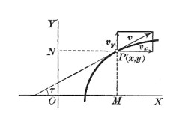
\includegraphics[height=3cm,width=5cm]{vel-comps.eps}
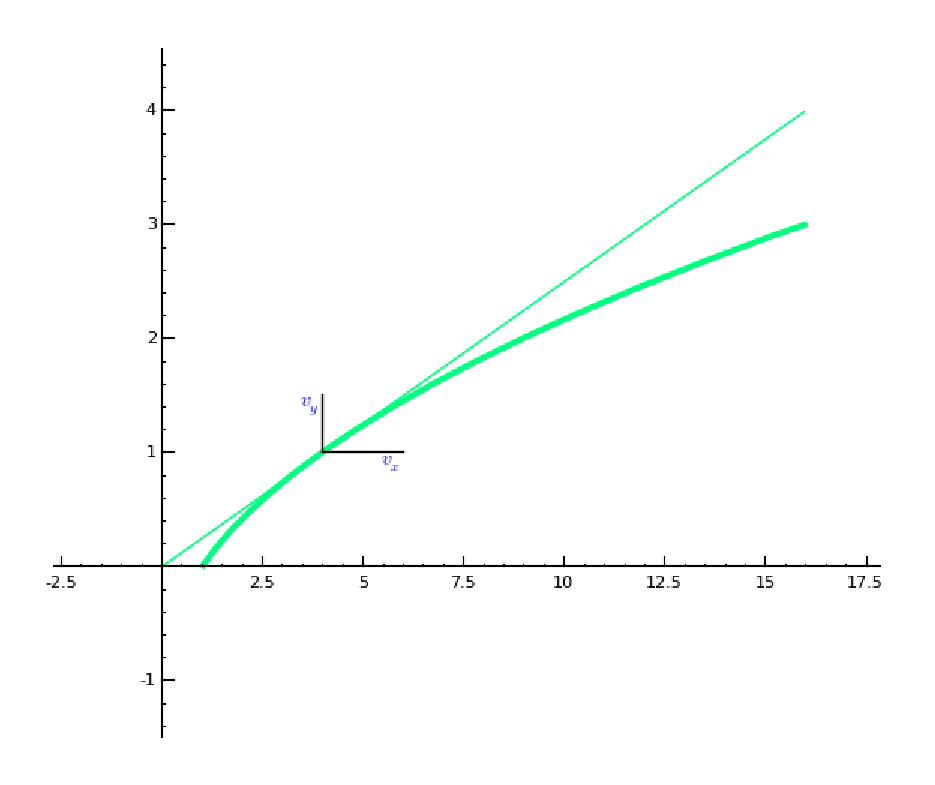
\includegraphics[height=5cm,width=8cm]{vel-comps2.eps}
\end{center}
\end{minipage}
%\caption{Scan of Granville's graphic of the components of velocity.}
\caption{The components of velocity.}
\label{fig:vel-comps}
\end{figure}


The horizontal component\footnote{The direction of $v$ is along 
the tangent to the path.}
$v_x$ of $v$ is the velocity along the $x$-axis of 
the projection M of P, and is therefore the time rate of change of $x$. 
Hence, from (\ref{eqn:9-70}), %p. 90 [§70], 
when $s$ is replaced by $x$, we get

\begin{equation}
%(10) 
v_x = \frac{dx}{dt}.
\label{eqn:10-71}
\end{equation}	
In the same way we get the vertical component, or time rate of change of $y$,

\begin{equation}
%(11) 
v_y = \frac{dy}{dt}.
\label{eqn:11-71}
\end{equation}	
Representing the velocity and its components by vectors, we have at once from the figure

\[
    v^2 = {v_x}^2 + {v_y}^2,
\]
or,

\begin{equation}
%(12) 
v = \frac{ds}{dt} 
= \sqrt{\left ( \frac{dx}{dt} \right )^2 + \left ( \frac{dy}{dt} \right )^2},
\label{eqn:12-71}
\end{equation}	
giving the magnitude of the velocity at any instant.

If $\tau$ be the angle which the direction of the velocity makes 
with the $x$-axis; we have from the figure, using (\ref{eqn:9-70}), 
(\ref{eqn:10-71}), (\ref{eqn:11-71}),

\begin{equation}
%(13) 
\sin \tau = \frac{v_y}{v} 
= \frac{\frac{dy}{dt}}{\frac{ds}{dt}}; \ \ 
\cos \tau = \frac{v_x}{v} = \frac{\frac{dx}{dt}}{\frac{ds}{ds}}; 
\ \ \tan \tau = \frac{v_y}{v_x} = \frac{\frac{dy}{dt}}{\frac{dx}{dt}}.
\label{eqn:13-71}
\end{equation}

%72. 
\section{Acceleration. Rectilinear motion.} 

In general, $v$ will be a function of $t$. 
%and we may write $v = \psi (t)$.
Now let $t$ take on an increment $\Delta t$, then $v$ takes 
on an increment $\Delta v$, and
$\frac{\Delta v}{\Delta t}$ is the average acceleration of 
P during the time interval $\Delta t$.
We define the {\it acceleration} $a$ at any instant as the 
limit of the ratio $\frac{\Delta v}{\Delta t}$ as $\Delta t$ approaches 
the limit zero; that is,
\index{acceleration}

\[
a = \lim_{\Delta t \to 0} \left ( \frac{\Delta v}{\Delta t} \right ),
\]
or,

\begin{equation}
%(14) 
a = \frac{dv}{dt}
\label{eqn:14-72}
\end{equation}
{\it The acceleration is the derivative of the velocity with respect to time.}

%73. 
\section{Component accelerations. Curvilinear motion.} 

In treatises on Mechanics it is shown that in curvilinear 
motion the acceleration is not, like the velocity, directed 
along the tangent, but toward the concave side, of the path of 
motion. It may be resolved into a tangential component, 
$a_t$, and a normal component, $a_n$ where

\begin{equation}
%(14a) 
a_t = \frac{dv}{dt};\ \ \  a_n = \frac{v^2}{R}.
\label{eqn:14a-73}
\end{equation}
($R$ is the radius of curvature. See \S \ref{sec:103}.) %§103.)

The acceleration may also be resolved into components parallel 
to the axes of the path of motion. Following the same plan used in 
\S \ref{sec:71} %§ 71 
for finding component velocities, we define the component 
accelerations parallel to the $x$-axis and $y$-axis,

\begin{equation}
%(15) 
a_x = \frac{dv_x}{dt}; \ \ \ \ a_y = \frac{dv_y}{dt}. 
\label{eqn:15-73}
\end{equation}
Also,
\begin{equation}
%(16) 
a = \sqrt{\left ( \frac{dv_x}{dt} \right )^2 + \left ( \frac{dv_y}{dt} \right )^2},
\label{eqn:16-73}
\end{equation}
which gives the magnitude of the acceleration at any instant.

\section{Examples}

\begin{enumerate}
\item
%1
By experiment it has been found that a body falling 
freely from rest in a vacuum near the earth's surface follows 
approximately the law $s = 16.1t^2$, where $s$ = space (height) in feet, 
$t$ = time in seconds. Find the velocity and acceleration 

\begin{itemize}
\item[(a)] 
at any instant; 

\item[(b)]
at end of the first second; 

\item[(c)]
at end of the fifth second.
\end{itemize}

Solution. We have $s = 16.1t^2$.

(a) Differentiating, $\frac{ds}{dt} = 32.2 t$, or, from 
(\ref{eqn:9-70}), $v = 32.2t$ ft./sec.
Differentiating again, $\frac{dv}{dt} = 32.2$, or, from 
(\ref{eqn:14-72}), 
$a = 32.2\  \fps2$,
which tells us that the acceleration of a falling body 
is constant; in other words, the velocity increases $32.2$ ft./sec. 
every second it keeps on falling.

(b) To find $v$ and $a$ at the end of the first second, substitute 
$t = 1$ to get $v = 32.2$ ft./sec., $a = 32.2\  \fps2$.

(c) To find $v$ and $a$ at the end of the fifth second, 
substitute $t = 5$ to get $v = 161$ ft./sec., 
$a = 32.2\  \fps2$.

\item
%2
Neglecting the resistance of the air, the equations of motion for a 
projectile are

\[
x = v_0 \cos \phi \cdot t,\ \ \  y = v_0 \sin \phi \cdot t - 16.1 t^2;
\]
where $v_0$ = initial velocity, $\phi$ = angle of projection with 
horizon, $t$ = time of flight in seconds, $x$ and $y$ being 
measured in feet. Find the velocity, acceleration, component velocities, 
and component accelerations 

\begin{itemize}
\item[(a)] 
at any instant; 

\item[(b)]
at the end of the first second, having given $v_0 = 100$ ft. per sec., 
$\phi = 30^0 = \pi/6$; 

\item[(c)]
find direction of motion at the end of the first second.
\end{itemize}

Solution. From (\ref{eqn:10-71}) and (\ref{eqn:11-71}),
(a) $v_x = v_0 \cos \phi$; \ $v_y = v_0 \sin \phi - 32.2 t$.
Also, from (\ref{eqn:12-71}), 
$v = \sqrt{{v_0}^2 - 64.4 t v_0 \sin \phi + 1036.8 t^2}$.
From (\ref{eqn:15-73}) and (\ref{eqn:16-73}), 	
$a_x = 0$; $a_y = − 32.2$; $a =  32.2$.

(b) Substituting $t = 1$, $v_0 = 100$, $\phi = 30^0=\pi/6$ in these 
results, we get
  	$v_x = 86.6$ ft./sec., $a_x = 0$;
  	$v_y = 17.8$ ft./sec., $a_y = - 32.2\ \fps2$;
  	$v = 88.4$ ft./sec., $a = 32.2\ \fps2$.

(c) 	
$\tau = \arctan \frac{v_y}{v_x} = \arctan \frac{17.8}{86.6} = 0.2027...
\approx 11^o$, which is the angle of direction of motion with the horizontal.

\item
%3
Given the following equations of rectilinear motion. 
Find the distance, velocity, and acceleration at the instant indicated:

\begin{itemize}
\item[(a)] 
$s = t^3 + 2t^2$; $t = 2$. 	

Ans. 	$s = 16$, $v = 20$, $a = 16$.

\item[(b)] 

$s = t^2 + 2t$; $t = 3$. 	

Ans. $s = 15$, $v = 8$, $a = 2$.

\item[(c)] 
$s = 3 - 4t$; $t = 4$. 	

Ans. $s = - 13$, $v = - 4$, $a = 0$.

\item[(d)] 
$x = 2t - t^2$; $t = 1$. 	

Ans. $x = 1$, $v = 0$, $a = - 2$.

\item[(e)] 
$y = 2t - t^3$; $t = 0$. 	

Ans. $y = 0$, $v = 2$, $a = 0$.

\item[(f)] 
$h = 20t + 16t^2$; $t = 10$. 	

Ans. $h = 1800$, $v = 340$, $a = 32$.

\item[(g)] 
$s = 2 \sin\, t$; $t = \frac{\pi}{4}$. 	

Ans. $s = \sqrt{2}$, $v = \sqrt{2}$, $a= - \sqrt{2}$.

\item[(h)] 
$y = a \cos \frac{\pi t}{3}$; $t = 1$. 	

Ans. $y = \frac{a}{2}$, $v = -\frac{\pi a \sqrt{3}}{6}$, $a = -\frac{\pi^2 a}{18}$.

\item[(i)] 
$s = 2e^{3t}$; $t = 0$. 	

Ans. $s = 2$, $v = 6$, $a = 18$.

\item[(j)] 
$s = 2t^2 - 3t$; $t = 2$.

\item[(k)] 
$x = 4 + t^3$; $t = 3$.

\item[(l)] 
$y = 5 \cos\, 2t$; $t = \frac{\pi}{6}$.

\item[(m)] 
$s = b \sin \frac{\pi t}{4}$; $t = 2$.

\item[(n)] 
$x = ae^{- 2t}$; $t = 1$.

\item[(o)] 
$s = \frac{a}{t} + bt^2$; $t = t_0$.

\item[(p)] 
$s = 10 \log \frac{4}{4 + t}$; $t= 1$.

\end{itemize}

\item
%4
 If a projectile be given an initial velocity of $200$ ft. per sec. 
in a direction inclined $45^o=\pi/4$ with the horizontal, find

\begin{itemize}
\item[(a)] 
the velocity and direction of motion at the end of the third and sixth seconds;

\item[(b)] 
the component velocities at the same instants.
\end{itemize}

Conditions are the same as for Exercise 2.

Ans. 	
\newline
(a) 	When $t = 3$, 	$v = 148.3$ ft. per sec., $\tau = 0.3068... = 17^o 35'$;
when $t = 6$, $v = 150.5$ ft. per sec., $\tau = 2.79049... = 159^o 53'$;

(b) When $t = 3$, $v_x = 141.4$ ft. per sec., $v_y = 44.8$ ft. per sec.;
when $t = 6$, $v_x = 141.4$ ft. per sec., $v_y = - 51.8$ ft. per sec.

\item
%5
The height (= $s$) in feet reached in $t$ seconds by a body 
projected vertically upwards with a velocity of $v_0$ ft. per sec. 
is given by the formula
$    s = v_0t - 16.1t^2$.
Find 

(a) velocity and acceleration at any instant; and, if 
$v_0 = 300$ ft. per sec., find velocity and acceleration 

(b) at end of 2 seconds; 

(c) at end of 15 seconds. Resistance of air is neglected.

Ans. 	(a) $v = v_0 - 32.2t$, $a = - 32.2$;
  	(b) $v = 235.6$ ft. per sec. Upwards,
  	$a = 32.2$ ft. per (sec.)$^2$ downwards;
  	(c) $v = 183$ ft. per sec. Downwards,
  	$a = 32.2$ ft. per (sec.)$^2$ downwards.

\item
%6
A cannon ball is fired vertically upwards with a muzzle 
velocity of $644$ ft. per sec. Find (a) its velocity at the end of 
$10$ seconds; (b) for how long it will continue to rise. 
Conditions same as for Exercise 5.

Ans. (a) $322$ ft. per sec. Upwards; (b) $20$ seconds.

\item
%7
A train left a station and in $t$ hours was at a distance (space) of

\[
 s = t^3 + 2t^2 + 3t
\]
miles from the starting point. Find its acceleration 
(a) at the end of $t$ hours; (b) at the end of $2$ hours.

Ans. 	(a) $a = 6t + 4$; (b) $a = 16$ miles/(hour)$^2$.
\item
%8
In $t$ hours a train had reached a point at the distance of 
$\frac{1}{4} t^4 - 4t^3 + 16t^2$ miles from the starting point. 

\begin{itemize}
\item[(a)] 
Find its velocity and acceleration. 

\item[(b)] 
When will the train stop to change the direction of its motion? 

\item[(c)] 
Describe the motion during the first 10 hours.
\end{itemize}

Ans. 	(a) $v = t^3 - 12t^2 + 32t$, $a = 3t^2 - 24t + 32$;

  	(b) at end of fourth and eighth hours;

  	(c) forward first $4$ hours, backward the next $4$ hours, 
forward again after $8$ hours.

\item
%9
The space in feet described in $t$ seconds by a point is expressed by the formula

\[
 s = 48t - 16t^2.
\]
Find the velocity and acceleration at the end of 
$\frac{3}{2}$ seconds.

Ans. $v = 0$,$a = - 32\ \fps2$.

\item
%10
 Find the acceleration, having given

\begin{itemize}
\item[(a)] 
$v = t^2 + 2t$; $t = 3$. 	

Ans. 	$a = 8$.

\item[(b)] $v = 3t- t^3$; $t = 2$. 

Ans. $a = - 9$.

\item[(c)] $v = 4 \sin \frac{t}{2}$; $t = \frac{\pi}{3}$. 

Ans. $a = \sqrt{3}$.

\item[(d)] $v = r \cos\, 3t$; $t = \frac{\pi}{6}$.

Ans. $a = - 3r$.

\item[(e)] $v = 5e^{2t}$; $t = 1$. 

Ans. $a = 10e^2$.
\end{itemize}

\item
%11
At the end of $t$ seconds a body has a velocity of 
$3t^2 + 2t$ ft. per sec.; find its acceleration (a) in general; 
(b) at the end of $4$ seconds.

Ans. (a) $a = 6t + 2\ \fps2$; (b) 
$a = 26\ \fps2$
\item
%12
The vertical component of velocity of a point at the end of 
$t$ seconds is

\[
 v_y = 3t^2 - 2t + 6 
\]
in ft. per sec.
Find the vertical component of acceleration (a) at any instant; 
(b) at the end of $2$ seconds.

Ans. (a) $a_y = 6t - 2$; (b) $10\ \fps2$ .

\item
%13
 If a point moves in a fixed path so that

\[
 s = \sqrt{t},
\]
show that the acceleration is negative and proportional to the 
cube of the velocity.

\item
%14
 If the distance travelled at time $t$ is given by

\[
s = c_1e^t + c_2e^{-t},
\]
for some constants $c_1$ and $c_2$,
show that the acceleration is always equal in magnitude to the space 
passed over.

\item
%15
 If a point referred to rectangular coordinates moves so that

\[
x = a_1+a_2\cos\,t , \ \ \ y = b_1+b_2\sin\, t ,
\]
for some constants $a_i$ and $b_i$,show that its velocity has a 
constant magnitude.

\item
%16
 If the path of a moving point is the sine curve

\[
\begin{cases} 
x = at, \\ 
y = b \sin\, at 
\end{cases}
\]
show (a) that the $x$-component of the velocity is constant; (b) that 
the acceleration of the point at any instant is proportional 
to its distance from the $x$-axis.

\item
%17
Given the following equations of curvilinear motion, 
find at the given instant 

\begin{itemize}
\item
$v_x$, $v_y$, $v$;
\item
$a_x$, $a_y$, $a$; 
\item
position of point (coordinates); 
\item
direction of motion. 
\item
the equation of the path in rectangular coordinates.
\end{itemize}

\begin{itemize}
\item[(a)] 
$x = t^2$, $y = t$; $t = 2$.

\item[(g)] 
$x = 2\sin\, t$, $y = 3\cos\, t$; $t = \pi$.

\item[(b)] 
$x = t$, $y = t^3$; $t = 1$.
 	
\item[(h)] 
$x = \sin\, t$, $y = \cos\, 2t$; $t = \frac{\pi}{4}$.

\item[(c)] 
$x = t^2$, $y = t^3$; $t = 3$.
 	
\item[(i)] 
$x = 2t$, $y = 3e^t$; $t = 0$.

\item[(d)] 
$x = 2t$, $y = t^2 + 3$; $t = 0$.

\item[(e)] 
$x = 1 - t^2$, $y = 2t$; $t = 2$.
 	
\item[(j)] 
$x = 3t$, $y = \log\, t$; $t = 1$.

\item[(f)] 
$x = r \sin\, t$, $y = r \cos\, t$; 
$t = \frac{3\pi}{4}$.
 	
\item[(k)] 
$x = t$, $y = 12/t$; $t = 3$.

\end{itemize}

\end{enumerate}

